\documentclass[11pt]{report}
\usepackage{standalone}
\graphicspath{ {images/} }
\setcounter{tocdepth}{5}
\setcounter{secnumdepth}{5}
\usepackage{natbib}
\usepackage{bibentry}
\bibliographystyle{agsm}
\usepackage{etoolbox}
\setlength{\parindent}{0em}
\setlength{\parskip}{0.25em}
\usepackage[raggedright]{titlesec}
\usepackage{hyperref}
\usepackage{capt-of}
\patchcmd{\bibliography}{\section*}{\section}{}{}
\titlespacing*{\chapter}{0pt}{-40pt}{10pt}
\titleformat{\chapter}[block]{\normalfont\huge\bfseries}{\thechapter}{15pt}{}
\usepackage{rotating}
\usepackage[titletoc]{appendix}
\usepackage{pgfgantt}
\usepackage{graphicx, rotating, caption, lscape, threeparttable}% \usepackage{amsmath}
\usepackage{array}
\usepackage{pdflscape}
\usepackage{geometry}
\usepackage{listings}
\usepackage[T1]{fontenc}
\usepackage[bottom]{footmisc}
\usepackage{multirow}
\usepackage{float}
\usepackage{subcaption}
\usepackage{textcomp}
\usepackage{etoolbox}
\usepackage{epigraph}

\setlength\epigraphwidth{11cm}
\setlength\epigraphrule{0pt}
\makeatletter
\patchcmd{\epigraph}{\@epitext{#1}}{\itshape\@epitext{#1}}{}{}
\makeatother




  
\begin{document}
\documentclass[11pt]{article}
\usepackage{graphicx}
\usepackage{pgfgantt}
\usepackage{soul}% Increases your ability to emphasize text
\graphicspath{ {images/} }

\begin{document}

\begin{titlepage}

\newcommand{\HRule}{\rule{\linewidth}{0.5mm}} % Defines a new command for the horizontal lines, change thickness here

\center % Center everything on the page
 
%----------------------------------------------------------------------------------------
%   HEADING SECTIONS
%----------------------------------------------------------------------------------------

\textsc{
	\LARGE University Of Birmingham\\
	\vspace{5mm}
	\large School Of Computer Science
}\\[1.5cm] % University Of Birmingham
\textsc{\Large Dissertation Report}\\[0.5cm]

%----------------------------------------------------------------------------------------
%   TITLE SECTION
%----------------------------------------------------------------------------------------

\HRule \\[0.4cm]
{ \huge \bfseries A Real Time System for the Sentiment Analysis of the Brexit Twitter
Debate}\\[0.4cm] % Title of your document
\HRule \\[1.5cm]
 
%----------------------------------------------------------------------------------------
%   AUTHOR SECTION
%----------------------------------------------------------------------------------------

\begin{minipage}{0.4\textwidth}
\begin{flushleft} \large
\emph{Author:}\\
Brad \textsc{Rowe} \\
\end{flushleft}
\end{minipage}
~
\begin{minipage}{0.4\textwidth}
\begin{flushright} \large
\emph{Supervisor:} \\
Dr. Phillip \textsc{Smith} % Supervisor's Name
\end{flushright}
\end{minipage}\\[0.5cm]

\begin{minipage}{1\textwidth}
\begin{center} \large
\emph{Programme:} \\
BSc Computer Science with Industrial Year 
\end{center}
\end{minipage}\\[0.5cm]


% If you don't want a supervisor, uncomment the two lines below and remove the section above
%\Large \emph{Author:}\\
%John \textsc{Smith}\\[3cm] % Your name

%----------------------------------------------------------------------------------------
%   DATE SECTION
%----------------------------------------------------------------------------------------
\vspace{1cm}

{\large \today}\\[0.75cm] % Date, change the \today to a set date if you want to be precise

%----------------------------------------------------------------------------------------
%   LOGO SECTION
%----------------------------------------------------------------------------------------

\includegraphics[width=4.5cm, height=5cm]{logo}
 
%----------------------------------------------------------------------------------------

\vfill % Fill the rest of the page with whitespace

\end{titlepage}
\end{document}

\clearpage
\chapter*{\centerline{Preamble}}
\addcontentsline{toc}{chapter}{Preamble}
\vspace{1cm}

\section*{\centering Abstract}
\addcontentsline{toc}{section}{Abstract}
Political Opinion; traditionally extrapolated from polling data has since seen a developing trend into the utilisation of sentiment analysis on freely available social media data as a means of gaining further opinion insights. This paper draws on the previous work into political analysis via statistical sentiment extraction and henceforth investigates whether `we can implement an autonomous system to extract and visualise public sentiment from Tweets within sufficient real time'. Using user posted twitter data on the discussion of `Britain leaving the European Union' as a case study pertinent to the question posed. Previous work into the extraction of political opinion via Twitter have failed to utilise the power of Neural Networks as deep learning tools to aid in the extraction of contextual sentiment. Furthermore, in the case study of `Britain Leaving the European Union' previous systems have trivially extracted sentiment by not using Neural Networks and have thus failed to acknowledge the importance of ``context'' within a domain specific text like online political discourse. 

\vspace{0.5cm}
\begin{center}
\section*{\centering Git Repository}
\addcontentsline{toc}{section}{Git Repository}
All Software and Documentation within this Report can be found at: \\
\medskip
\href{https://git-teaching.cs.bham.ac.uk/mod-ug-proj-2017/bmr455/}{https://git-teaching.cs.bham.ac.uk/mod-ug-proj-2017/bmr455/}
\end{center}

\vspace{0.5cm}
\section*{\centering Acknowledgements}
\addcontentsline{toc}{section}{Acknowledgements}
I would like to express a token of appreciation to my supervisor Dr.\ Phillip Smith, for his guidance and support within the development of the project. His   supervisory time and passion for the subject influenced the outcome of the project significantly and for that I am especially grateful. 
\clearpage
\tableofcontents





\chapter{Introduction}
\documentclass[11pt]{report}
\usepackage{etoolbox}
\usepackage{epigraph}

\setlength\epigraphwidth{\textwidth}
\setlength\epigraphrule{0pt}
\makeatletter
\patchcmd{\epigraph}{\@epitext{#1}}{\itshape\@epitext{#1}}{}{}
\makeatother


\begin{document}
  
\section{Problem}
For long, as individuals we have chosen to express our beliefs and experiences through the medium of written word. Within recent years social media has become ubiquitous in our daily lives, and with that has become a growing trend to share our thoughts in online \textit{posts}. The Question arises then on whether sentiment analysis of \textit{posts such as tweets} can be used to provide a clearer understanding of what sentiment is expressed within a domain context such as the political area of debate regarding  ``Britain Leaving the European Union'' via Twitter. More specifically the problem for which this report aims to tackle is whether the sub-tasks of classifying sentiment can be automated and combined with visualization to form a system that can computationally analyse the sentiment of a domain context within real-time.
 
\section{Context}
Despite the act of Britain voting to leave the European Union dating back almost two years at publishing date of this report, it remains a hot topic in the forum of online social media. Discussions have now turned towards the opinion on the execution of Article 50 during the negotiation period that Britain currently finds itself in. Online discourse regarding ``Britain Leaving the European Union'' (also referred to as Brexit) has been and will continue to be a rich source of public opinion and as a consequence solidifies the grounds for extracting sentiment on the matter of which this report goes on to discuss.

\clearpage
\section{Overview}
\subsection*{Project Scope}
The work as outlined by this Report first and foremost provides a software system that can be used to extract and visualize the sentiment of tweets within real time. Secondly, it builds on existing work regarding the case study of "Britain leaving the European Union" using tweets belonging to the wider discussion of the topic. Through practical application of the system using the case study as mentioned the by-products have been further work into investigating to what extent sentiment analysis can be used as a method for political social media opinion mining and new insights into general public consensus on "Britain Leaving the European Union" since the EU Referendum public vote.

\subsection*{Report}
The following sections of the report detail the system and the rationale behind the design, implementation and evaluation of this class of system. To summarize the report will proceed as follows:

\begin{itemize}

\item Related Work - Summary of existing work within the domain area's for which this unit of work explores.

\item Analysis - The analysis of the problem that was undertaken consisting of a system specification and requirements of the system.

\item Design - The rationale behind the architecture of the system and the visual stimuli for which the user interfaces with the system.

\item Project Management - The techniques utilized in managing the development and execution of the project.

\item Implementation - How the solution operates, the application programming interfaces used and a summary of the technology required.

\item Experiments and Testing - a report of the testing carried out as part of the System's development.

\item Discussion - Qualitative and quantitative review of the System, it's performance and proposed future extensions.

\item Conclusion - Summary of the work outlined in this report.
\end{itemize}

\end{document}

\documentclass[11pt]{report}
\usepackage{standalone}
\graphicspath{ {images/} }
\setcounter{tocdepth}{5}
\setcounter{secnumdepth}{5}
\usepackage{natbib}
\bibliographystyle{agsm}
\usepackage{etoolbox}
\setlength{\parindent}{0em}
\setlength{\parskip}{0.25em}
\usepackage[raggedright]{titlesec}
\usepackage{hyperref}
\usepackage{capt-of}
\patchcmd{\bibliography}{\section*}{\section}{}{}
\titlespacing*{\chapter}{0pt}{-40pt}{10pt}
\titleformat{\chapter}[block]{\normalfont\huge\bfseries}{\thechapter}{15pt}{}
\usepackage{rotating}
\usepackage[titletoc]{appendix}
\usepackage{pgfgantt}
\usepackage{graphicx, rotating, caption, lscape, threeparttable}% \usepackage{amsmath}
\usepackage{array}
\usepackage{pdflscape}
\usepackage{geometry}
\usepackage{listings}
\usepackage[T1]{fontenc}


\begin{document}
\chapter{Related Work}
\label{chap:related-work}

\section{Sentiment Analysis Background}
Historically Opinion Mining and Sentiment Analysis (OMSA) of a computer based nature arose as a method to gain further insight into ``Customer Reviews'' in the commercial markets of movies \citep{turney_thumbs_2002, hu_mining_2004} and products \citep{morinaga_mining_2002, popescu_extracting_2005}.  As \cite{cambria_new_2013} states \lq{The Web has changed from ``read-only'' to ``read-write''}\rq and what came of this change was an increasing amount of user engagement with websites, blogs, forums and social media all of which lend themselves to being a rich source of public opinion. 

\subsection*{Approaches to Sentiment Extraction}
In literature, the common underpinnings of research towards sentiment extraction follow a rule based or statistical approach with some scholars combining the two. Early rule based approaches employed the creation and usage of context-free rules independent of the domain in which they are investigating \citep{read_weakly_2009}. These approaches used prior polarity to determine semantic orientation using generated lexicons \citep{TaboadaLexiconbasedMethodsSentiment2011} as well as the likes of established lexicons; SentiWordNet \citep{esuli_sentiwordnet:_2006}, the General Inquirer \citep{stone_computer_1963} and Maryland \citep{mohammad_generating_2009} to name just a few. The weaknesses as highlighted by \cite{TaboadaLexiconbasedMethodsSentiment2011} is that the ``coverage'' of these lexicons are too generic and fail to aid in sentiment extraction of texts for which the sentiment lies in the domain from where they are sourced. For instance, the word `long' may have positive sentiment when discussing the life-span of product i.e. `this watch is well built and will last long' however when applied to the context of a movie i.e. `the movie was long and tedious' the same phrase would carry a negative sentiment. This contrast of sentiment between domains leads to poor generalization when applying context-free lexicons like the aforementioned to a domain text. This therefore prompted further research into corpus based lexicons; \cite{cho_data-driven_2014} found the reduction of a lexicon's size and reclassifications of it' contained sentiment polarities with respect to domain led to an overall improvement in accuracy of sentiment classification. Having derived that a lexical approach towards sentiment extraction of a domain specific corpus performs poorly and how \cite{read_weakly_2009} hypothesizes `with regards to topic and temporal dependency, it is still more effective to use supervised machine learning and accept some loss in performance when analysing data of a different topic or time-period' and thus the domain and temporal research as outlined by this paper extends on the supervised statistical approach towards sentiment extraction.

\section{Sentiment Analysis on Twitter}
More recently in the field of OMSA, research has been led into the user engagement of Social Media more specifically Twitter with a total of 11.06\% of recent research papers (2000-2015) containing twitter datasets \citep{piryani_analytical_2016}. Twitter as a platform originally intended for user conversations has since developed into a social hub of subjective opinions due to the paradigm `shift from traditional communication tools (such as traditional blogs or mailing lists) to microblogging services' \citep{pak_twitter_2010}. With the rise of ubiquity in microblogging among society and the ever-growing channels of discussion on Twitter, a wealth of opinion has been conceived thus presenting opportunism for new insights into a plethora of topical public opinion.

\subsection*{Areas of Focus}
The nature of previous OMSA twitter studies have varied as Twitter has evolved to become a leading online platform for short-informal communication. Again, the same early commercial motives of sentiment extraction can be seen in Twitter OMSA; studies into consumer brand opinion extraction have used lexicon's compromised of uni-grams and bi-grams with each having an associated positive and negative polarity distribution. \cite{jansen_twitter_2009} were able to use such a lexicon to classify a tweet on a five-point scale using a multinomial statistical Bayes model approach. However, there are numerous nonprofit Twitter sentiment extraction studies focused on past and present topics. These studies typically aim to provide clarity on investigatory topics as well as building effective models in predicting future outcomes using twitter encapsulated entities as data to explore these aims. One such noteworthy study by \cite{bollen_modeling_2009} investigated the correlation of collective mood changes on Twitter with social, economic and political events. The study uses previous work of extracting sentiment using an adapted physcometric profile of mood states test \citep{pepe_between_2008} to model the time series standard deviations on a six-point-mood-scale towards socio economic phenomena. Interestingly the results found by  \cite{bollen_modeling_2009} were `events in the social, political, cultural and economical sphere do have a significant, immediate and highly specific effect on the various dimensions of public mood' with public mood deviations varying the most from `short-term events such as the news cycle, elections, national holidays, and other events' compared that of long term economic events where public mood `changes seem to have a more gradual and cumulative effect'. The investigation into twitter discourse regarding socio economic phenomena therefore has substance in extracting directly affected public opinion. And it is this observation of linkage between socio economic events and twitter sentiment which is pertinent to this papers investigatory aims of extracting public opinion regarding Britain leaving the European Union using tweets from the eventful temporal window after the `eu-referendum results'. 

\subsection*{Approaches to Sentiment Extraction}
Twitter Sentiment Analysis studies have seen significant work on classifying tweets or other twitter encapsulated entities with respect to binary and multinomial classifications such as the determination of a tweet's polarity. The structure of supervised Twitter OMSA work have commonality in the following; the data is typically preprocessed, the classification algorithms are refined through experiments using labelled training samples and the evaluation metrics of the final model are reported. The limitations of such a supervised model can be seen to be somewhat linked to the limitations of the available dataset. This assumption has been evidenced in Twitter such that the limitation in size of a dataset has been revealed to directly impact the performance accuracy of sentiment classifiers \citep{pak_twitter_2010}, however it is not the case that the size of dataset and performance accuracy are proportionally linked as the performance gain tapers off after the dataset is large enough. The maxima of performance gain from the size of data is arguably the point of vocabulary convergence where unseen samples can be accurately classified from a diverse and representative training set. Despite individuals casting their own opinion, it's argued that opinions of a topical context `converge' in the language and points for which their opinion contains; \citep{hu_mining_2004} and \citep{wu_exploration_2011} highlight this point of convergence in online discourse for products and political events respectively. Further to size; the correct labelling of a training set is key to producing an optimal classifier. Smaller studies into extracting sentiment through twitter have used manual approaches towards labelling data, however this as a practice is susceptible to introducing bias into the training of a model. Even if bias is removed through cross-labelling techniques the manual nature ceases to be a viable when having to manually annotate large numbers of samples which as highlighted before is needed to produce optimal accuracy. Instead, various studies have took an automated approach to labelling using distant supervision on large scale training sets. These studies have implemented automated labelling through `noisy labels' such as the use of hashtags \cite{} and emojis \citep{jonathon_using_2005} to act as the label for the semantic orientation of a tweet. Having deduced that an optimal model of sentiment extraction within Twitter is depdendent on the representative size and labelling of it's training set, the partitioning and labelling of this paper's training set will be carried out using automated labelling influenced by the established techniques of utilizing textual content of a tweet to procure it's label.

\section{Sentiment Analysis of Political Discourse on Twitter}
The reactive nature of Twitter sentiment to socio economic phenomena as evidenced above has thus led to a growing number of studies into extracting sentiment on global political affairs.
\subsection*{Twitter as a viable source for extracting political sentiment}
Public Opinion on political affairs has long been analysed using traditional polling methods. Although traditional methods are manual and costly to carry out, over time they have had significant scientific backing to ensure the results obtained are representative and non-bias. The weakness of polls comes from the restrictiveness of specified questions and ensuring the sampling is completely representative of the nation. Here Twitter differs, the free-form nature provides access to new patterns and the nationwide usage can arguably give a representative sample of opinion from the nations younger demographic. Twitter sentiment analysis studies have echoed the results of traditional polls; \cite{tumasjan_predicting_2010} found that the share of messages regarding political parties in the 2009 German National parliament election was a close indicator of the true election results; predicting vote share within 1.65 percent mean absolute error across the parties.  \cite{jensen_psephological_2013} also hypothesized that the percentage of tweets regarding a political entity has some correlation to the percentage of a vote, using the 2012 Iowa elections as a case study they achieved 3.1 percent mean deviation from the true outcome differing by 1.1 percent from that of the 2.2 percent mean deviation of the traditional polls. It could thus be argued that tweet count can be considered an indicator for predicting vote share in upcoming elections however critics have questioned the validity of such studies with respect to the choice of datasets \citep{andreas_jungherr_why_2012}. Despite criticisms on validity these earlier political sentiment systems posed the question whether tweets could be used as an indicator of an individuals political sentiment. Divulging away from the simpler models of using tweet count as an indicator of election presence; there have been studies which have used more complex properties of twitter entities to aid in political classifications. \cite{pennacchiotti_machine_2011} used features such as; profile information, who a user follows, the textual content of a users tweets and the hashtags included in those tweets to classify a users political affiliation with either the Democrats or Republicans. \cite{pennacchiotti_machine_2011} achieved an average success rate over 80 percent across all of the features. Most notably from this case study it seemed that users of the same political affiliation tended to follow the same users, have similar textual content in their tweets and signed their tweets using similar hashtags.

\subsection*{Sentiment Analysis of Brexit}
Sentiment Analysis Classifiers in general benefit from clear cut orientations and political discourse is of no difference, whether it be the choice of an electoral candidate, the support towards a political party or an opinion on a political event by providing sentiments which are distinguishable i.e. the semantic orientations are different enough to warrant individual orientations, a classification to a higher then random level of accuracy can be made. One political movement which has embodied a strong polarisation in sentiments and is the topic of this paper for that very reason is Britain triggering article 50 to action it's exit from the European union or more commonly known as Brexit. The timeline of Britain leaving the European union can be naively split into three temporal windows; pre eu-referendum, the negotation period and Britain's exit from the European union.
\\

During the pre eu-referendum period the polling consensus was one of a majority support towards voting for Britain to remain in the European Union. However, \cite{porcaro_tweeting_2016} found that Twitter told a story contrary to this; it was discovered that a surge in pro-leave sympathies came in the summer of 2015 and remained persistently high up until the referendum. This contrast between the polls results and twitter is intriguing with twitter indicating the the true outcome much earlier it highlights the predictive power of twitter should not be underestimated. In addition, \cite{matsuo_more_2017} also found that the leave side dominated the twitter sphere; finding that the quantity of leave tweets was consistently higher up until election day where the remain side fought to be heard in a last ditch attempt to convince swing voters, that the leave side used more positive language when tweeting and that leave tweets tended to discuss the future with more certainty compared to the remain counterpart which spoke more on the past with a greater tentative tone. 
\\

Post eu-referendum, Britain and it's democratic leadership face negotiations to define the terms of Britain's exit from the European Union. Despite Britain having voted toward leaving the European Union the discussion of Brexit still remains an active channel of discussion within the twitter arena but few researchers have chosen to analyse the sentiment in situ of the negotiations. \cite{llewellyn_brexit?_2016} had produced a real time sentiment system which analysed the twitter discussion around Brexit in the run up to the referendum but have continued to run their system post eu-referendum. The Edinburgh system extracts sentiment towards the leave and remain stances, tracks trending hashtags and streams in the ongoing discussion as well as highlighting active locations of brexit related tweets all visible through daily and overview granularity. The Edinburgh system however trivially extracts sentiment using `the counts of human defined pro-Remain and pro-Leave hashtags' to signify sentiment towards the discussed brexit affiliation. Fundamentally, employing the count of a Brexit stance as the sentiment of said stance is a weak indicator of actual sentiment as tweets may critique a Brexit stance by mentioning it and not necessarily support the stance. \cite{maynard_framework_2017} real-time system also tracks Brexit stance sentiment but the Sheffield system differs from the Edinburgh system in that the system aims to analyse the topics discussed, the people involved in the discussion and opinions posted. The Sheffield system offers an improvement on the determination of a tweets Brexit stance; by using the presence of a pre-determined Brexit stance hashtag at the end position of a tweet the system can deduce the political stance of a given tweet. 
\\
\enlargethispage{\baselineskip}
\enlargethispage{\baselineskip}
\vspace{-0.20cm}

Being that the systems analysing the temporal window post referendum in situ are scarce and that the collective results of the above Systems leave room to provide incremental improvements in sentiment extraction; the System developed as part of this paper will capitalize on this and produce further insight into public opinion on the matter.
\end{document}

\documentclass[11pt]{report}
\usepackage{standalone}
\graphicspath{ {images/} }
\setcounter{tocdepth}{5}
\setcounter{secnumdepth}{5}
\usepackage{natbib}
\bibliographystyle{agsm}
\usepackage{etoolbox}
\setlength{\parindent}{0em}
\setlength{\parskip}{0.25em}
\usepackage[raggedright]{titlesec}
\usepackage{hyperref}
\usepackage{capt-of}
\patchcmd{\bibliography}{\section*}{\section}{}{}
\titlespacing*{\chapter}{0pt}{-40pt}{10pt}
\titleformat{\chapter}[block]{\normalfont\huge\bfseries}{\thechapter}{15pt}{}
\usepackage{rotating}
\usepackage[titletoc]{appendix}
\usepackage{pgfgantt}
\usepackage{graphicx, rotating, caption, lscape, threeparttable}% \usepackage{amsmath}
\usepackage{array}
\usepackage{pdflscape}
\usepackage{geometry}
\usepackage{listings}
\usepackage[T1]{fontenc}




\begin{document}
\chapter{Analysis}

\section{Requirements Elicitation}
To ensure the complete set of system requirements was gathered two methods of requirement capture were employed which include Observation and Inspection of Existing System Documentation. Each method allowed for the discovery of a smaller subset of requirements that when combined together gave a complete overview of what is required from the system.

\subsection*{Observation}
The existing Brexit visual sentiment system hosted by Edinburgh \citep{llewellyn_brexit?_2016} was observed to discover the core visual requirements of a semantic visualizer and areas of human computer interaction that required improvement in the Edinburgh system were noted as requirements of this system e.g. the granularity of different time levels rather than just having day and overview. 

\subsection*{Inspection of Existing System Documentation}
To gain an understanding of system features and what a classification framework requires, the existing documentation of real time classification system's by Edinburgh \citep{llewellyn_brexit?_2016} and Sheffield \citep{maynard_framework_2017} was analysed.

\section{Specification}
The requirements discovered within the requirements elicitation were formalised. Each of the requirements were then checked to ensure they were clear, unambiguous and verifiable. After which they were structured into the below software requirements specification.

\chapter*{Software Requirements Specification}

\subsection*{Product Functions}
\begin{itemize}
\item The System must be able to collect Tweets on the topic of ``Britain leaving the European Union''.
\item The System must be able to classify the sentiment of tweets that is has received.
\item The System must be able to visually display the sentiment of the public
on the topic of ``Britain leaving the European Union''.
\item The System must collect, classify and visualize the tweets within sufficient real time.
\item The System must be autonomous in it's operations.
\end{itemize}

\subsection*{User Classes and Characteristics}
\textbf{Operator}: An Individual who has a reasonable technical expertise and wants to interface with the System directly via command line tools and code itself.

\textbf{General User}: An individual who wishes to inspect the visual analysis that the system computes. This user is encompasses all the possible characteristics of a miscellaneous member of the general public wishing to engage with the system.

\subsection*{Operating Environment}
The System will operate on a remote virtual private server with an operating system of a Ubuntu Linux Distribution. 

The System will require a data store for permanent and temporary storage of data with the data store being maintainable, scalable and available at all times.

\subsection*{Design and Implementation Constraints}
There are a number of limiting factors that will constrain the Design and Implementation which are highlighted as follows:

External Storage Size: due to the system operating remotely the data store will also be remote and thus the amount of data stored will be a consideration.

RAM: the system may be operating on large amounts of data and thus must be conservative towards RAM usage at any one time.

Execution Time: the system collection, classification and visualization operations must occur within sufficient real time.

\subsection*{Dependencies}
The systems main dependency is Twitter, the system sources it's data from Twitter and thus the system, its successful delivery and continuous operation will require a reliable interface with Twitter itself.

\section*{External Interface Requirements}
\subsection*{Hardware Interfaces}
The System will have a visual website component (user interface) that will be developed to support all common device types from small constrained screen size devices such as mobile up to larger desktops.

\subsection*{Communications Interfaces}
\textbf{HTTP}: The System will require the use of HTTP connections for the consumption and exposure of data.

\textbf{SCP}: The System will require the use of the secure copy protocol for transferring the application files to the hosting destination of the remote virtual private server.

\subsection*{Interfaces}
The System will contain a command line interface and a visual interface for which the operator and general user will interact with respectively.

\subsubsection*{Command Line Interface}
The System will provide a command line interface for inputting commands within the system. Each component will have at least one runnable command e.g. for tweet collection component there will be commands for fetching historic tweets and fetching real time tweets. The main requirements of the set of these commands is that they must ensure user can view the progress of the command and that the user is presented with error messages where incorrect usage has occurred.
\\

\textbf{\underline{Progress}}

The execution time of commands may vary dependent on the command and the parameters given thus the system's operational commands must provide the user with a visual indication of progress.
\\

\textbf{\underline{Errors}}

Due to the commands being manually run the system will provide means of prompting the user with the correct parameter inputs i.e. a -h option for each command that informs the user of the required and optional parameters. The System should also inform the user of incorrect usage with commands.

\subsubsection*{Visual Website Interface}
The System's main user interface will be the visual website interface which will display all the tweets collected and the analysis conducted. 
\\

\textbf{\underline{Home View}}

This is the view in which new users will access the website from, the home page will introduce the key concepts of the site via text i.e. that the site is on the display of sentiment analysis and the site is looking at the discussion of ``Britain leaving the European Union'' via the forum of Twitter. The home page will also include the tweets for which it has most recently collected, the main navigation overlay to traverse the site and a button prompt to encourage users to read more on what the site is about.
\\

\textbf{\underline{About View}}

This is the view in which users will access when wanting to read more into how the site conducts it's analysis. The about page will clarify how the analysis was conducted from a high level and what important API's it uses in a tiled display fashion.
\\

\textbf{\underline{Analysis View}}

This is the view in which users will access when wanting to view the analysis conducted by the site, the analysis page will allow users to view analysis from the different classifications the system offers and give explanation behind each of the classifiers.
\\

\textbf{\underline{Classifier Analysis View}}

This is the view in which a user has selected a specific classifier they wish to view analysis for and are now presented with the analysis results. This view will display all the classifications for a given classifier and is viewable by time unit e.g. day/week/month/year. The view will allow for navigation by time unit using a time switcher group of buttons with a button for each of the aforementioned time units including forward and backward buttons to allow a user to go back/forth a time unit e.g. forward by one day would display the analysis of the next day after the currently selected one. Each time unit that has a lower granularity time unit represented by the system i.e. a week is composed of days, will provide the analysis of it's composite time units and provide buttons to view the analysis of each of them.

\clearpage
\section*{System Features}
Below is the catalogue of features that will be provided by the system, each feature contains it's summary description, available user interactions and it's measurable requirements.

\subsection*{1. Tweet Collection}
\subsubsection*{Feature Description}
The System must be able to collect, parse and save tweets that satisfy a selection criterion.
\subsubsection*{Stimulus/Response Sequences}
Using a command line interface; a user can give a selection criterion e.g. set of hashtags that tweets must contain and the system will collect tweets that satisfy that selection criterion.
\subsubsection*{Functional Requirements}
REQ-1.1:	The System must allow the user to specify hashtags for which to collect tweets for.

REQ-1.2: The System must collect tweets using it's given selection criterion.

REQ-1.3: The System must permanently store the tweets it collects.

\subsection*{2. Tweet Tokenization}
\subsubsection*{Feature Description}
The System must be able to tokenize tweets as part of a preprocessing step for classifications.
\subsubsection*{Stimulus/Response Sequences}
Using a command line interface; a user gives a tweet selection criteria, and the system will tokenize all tweets that satisfy the selection criteria and save the resulting tokenized tweets to the database.
\subsubsection*{Functional Requirements}
REQ-2.1: The System must provide an interface to allow users to manually tokenize tweets.

REQ-2.2: The System's tokenization interface must accept the user configurable input of a tweet selection criteria.

REQ-2.3: The System must be able to tokenize a plaintext tweet into a classifiable form.

REQ-2.4: The System must permanently store tokenized tweets that it has computed.
	
\subsection*{3. Tweet Classification}
\subsubsection*{Feature Description}
The System must be able to classify tweets against configurable classification models and store the resulting classifications for later use.
\subsubsection*{Stimulus/Response Sequences}
Using a command line interface; a user gives a selected classification model and tweet selection criteria, and the system will classify all tweets that satisfy the selection criteria and save the resulting classifications to the database.
\subsubsection*{Functional Requirements}
REQ-3.1: The System must provide an interface to allow users to manually classify tweets.

REQ-3.2: The System's classification interface must accept user configurable inputs of a tweet selection criteria and classification model.

REQ-3.3: The System must classify tweets on whether they are in favour (leave) or against (remain)  Britain Leaving the European union using brexit stance models.

REQ-3.4: The System must classify tweets on whether they are positive or negative towards Britain Leaving the European union using a sentiment polarity model.

REQ-3.5: The System must permanently store classifications that it has computed.


\subsection*{4. Visualization}
\subsubsection*{Feature Description}
The System must allow for the visualization of the tweets for which it has collected and the classifications for which it has computed.
\subsubsection*{Stimulus/Response Sequences}
Using the visualization interface a user can; 
\begin{itemize}
\item view tweets that the System has collected.
\item view the classifications that have been computed by each classification model within the System.
\item view the classifications the System has computed for a given classification model within a given time unit period.
\end{itemize}
\subsubsection*{Functional Requirements}
REQ-4.1: The System must display all Tweets that it has collected.

REQ-4.2: The System must provide a means of visually querying the resulting classifications by classification model.

REQ-4.3: The System must provide a means of visually querying the resulting classifications by time unit periods e.g. day/week/month/year.

REQ-4.4: The System must display all classifications and their associative tweets

\subsection*{5. Automation}
\subsubsection*{Feature Description}
The System must collect, tokenize, classify and visualize tweets autonomously.

\subsubsection*{Functional Requirements}
REQ-5.1: The System must conduct Tweet Collection autonomously.

REQ-5.2: The System must conduct Tweet Tokenization autonomously.

REQ-5.3: The System must conduct Tweet Classification autonomously.

REQ-5.4: The System must conduct Tweet Visualization autonomously.


\clearpage

\section*{Other Nonfunctional Requirements}
\subsection*{Performance Requirements}
NFREQ-1: The System must operate in real time and thus background operations must execute within an a max of an hour time window. 

NFREQ-2: The System must respond to HTTP Requests within 3 seconds.

\subsection*{Security Requirements}
The System will source its tweet data from the set of tweets which are publicly available or were publicly available at time of collection and thus the System abides by the twitter terms of service.

\subsection*{Software Quality Attributes}
NFREQ-3: The System must operate cross platform on the common operating systems e.g. Linux Distributions, Windows and Mac OSX.

NFREQ-4: The System visual interface must work across common browsers e.g. Safari, Chrome, Firefox and Opera.

NFREQ-5: The System must be flexible so that it operates as a framework allowing for classification models to be easily utilized in.

NFREQ-6: The System must be extensible in that the data models it stores are extendible.

NFREQ-7: The System should be reliably up and operating (and only down for when a new version is being deployed).

\end{document}

\documentclass[11pt]{report}
\usepackage{standalone}
\graphicspath{ {images/} }
\setcounter{tocdepth}{5}
\setcounter{secnumdepth}{5}
\usepackage{natbib}
\bibliographystyle{agsm}
\usepackage{etoolbox}
\setlength{\parindent}{0em}
\setlength{\parskip}{0.25em}
\usepackage[raggedright]{titlesec}
\usepackage{hyperref}
\usepackage{capt-of}
\patchcmd{\bibliography}{\section*}{\section}{}{}
\titlespacing*{\chapter}{0pt}{-40pt}{10pt}
\titleformat{\chapter}[block]{\normalfont\huge\bfseries}{\thechapter}{15pt}{}
\usepackage{rotating}
\usepackage[titletoc]{appendix}
\usepackage{pgfgantt}
\usepackage{graphicx, rotating, caption, lscape, threeparttable}% \usepackage{amsmath}
\usepackage{array}
\usepackage{pdflscape}
\usepackage{geometry}
\usepackage{listings}
\usepackage[T1]{fontenc}



\bibliographystyle{agsm}


\begin{document}
\chapter{Project Management}
\section{Development Methodology}
The project will take a sequential approach to the development process utilizing the waterfall model whose origins come from the seven stages of development conceived by \cite{RoyceManagingDevelopmentLarge1987}. The Waterfall model will ensure the project traverses through the software development lifecycle sequentially however as a contingency measure the model will be practised with feedback loops to ``go backwards in the software development lifecycle'' if the project requires it. The waterfall model which is suited to milestone-driven development will complement the project's timescale (see Figure \ref{fig:gantt}) and encourage the project to be structurally well designed before proceeding onto implementation phase of the development.

\section{Risk Analysis}
Throughout the project there are some risks which the development and progress of the project can be susceptible to. These risks should be dealt with correctly, and therefore a risk analysis plan has been documented as part of the planning within the project, Table \ref{table:risk-analysis} documents the main risks for which the project must plan against.

\section{Progress}
To ensure the project progresses and the system is delivered in full (all the identified requirements satisfied) the project milestones have been planned meticulously against the time available from inception to the completion of the project. Within the project timescale; weekly meetings with the project supervisor will occur to verify the project execution is on track and correct. An overview of the intended project timescale is covered within Figure \ref{fig:gantt}.

\clearpage

\newgeometry{a4paper,left=1in,right=1in,top=1in,bottom=1in,nohead}
\begin{landscape}
\begin{tabular}{ |>{\raggedright\arraybackslash}p{3cm}||p{3cm}|>{\raggedright\arraybackslash}p{5cm}|p{3cm}|>{\raggedright\arraybackslash}p{5cm}|  }
 \hline
 Risk & Likelihood & Effect & Strategy Type & Strategy Actions\\
  \hline
   Insufficient resources available & Highly likely & Progress is halted until resources available. & Avoidance & Where possible avoid resource intensive approaches i.e. complex infrastructure. \newline \newline Explore all possible approaches to resource intensive problems to ensure the most efficient approach for the available resources is chosen.\\
 \hline
 Complexity of Technology & Fairly likely & Slow down progress & Minimization & Avoid going too in-depth within complexities of technologies
 \newline \newline Read technology documentation where progress has slowed\\
  \hline
 Inadequate estimation of project timing & Unlikely & Reduce time available for remaining tasks & Contingency Plan & Re-adjust project timescale to ensure milestones have sufficient time to be met\\
  \hline
 Incorrect system requirements & Unlikely & Progress is halted until requirements are corrected & Contingency Plan & Reformulate requirements to ensure they are reflective of new observations. \\
 \hline
 Requirements Inflation & Unlikely & The quantitative amount of work required has increased & Minimization & Ensure the scope of each task is well defined \\
 \hline
\end{tabular}
\centering \captionof{table}{Project Risk Analysis Plan}
\label{table:risk-analysis}
\end{landscape}
\restoregeometry % Restore the global document page margins


\begin{center}
\resizebox{\textwidth}{!}{
\centering \begin{ganttchart}[
    canvas/.append style={fill=none, draw=black!5, line width=.75pt},
    hgrid style/.style={draw=black!5, line width=.75pt},
    vgrid={*1{draw=black!5, line width=.75pt}},
    title/.style={draw=none, fill=none},
    title label font=\bfseries\footnotesize,
    title label node/.append style={below=7pt},
    include title in canvas=false,
    bar label font=\mdseries\small\color{black!70},
    bar label node/.append style={left=0.5cm},
    bar/.append style={draw=none, fill=black!63},
    bar progress label font=\mdseries\footnotesize\color{black!70},
    group left shift=0,
    group right shift=0,
    group height=.5,
    group peaks tip position=0,
    group label node/.append style={left=.6cm},
    group progress label font=\bfseries\small,
    link/.style={-latex, line width=1.5pt, linkred},
    link label font=\scriptsize\bfseries,
    link label node/.append style={below left=-2pt and 0pt}
  ]{1}{25}
  \gantttitle[
    title label node/.append style={below left=7pt and -3pt}
  ]{WEEKS:\quad1}{1}
  \gantttitlelist{2,...,25}{1} \\
  \ganttgroup[]{1. Planning and Analysis}{1}{8} \\
  \ganttbar[
    name=1A
  ]{\textbf{1.1} Research Existing Systems/Resources}{1}{3} \\
  \ganttbar[
    name=1B
  ]{\textbf{1.2} Gather Requirements}{1}{3} \\
  \ganttbar[
    name=1C
  ]{\textbf{1.3} Project Proposal}{2}{4} \\
 \ganttbar[
    name=1D
  ]{\textbf{1.4} Literature Review}{4}{7} \\
  \ganttgroup[]{2. Design}{6}{8} \\
  \ganttbar[]{\textbf{2.1} System Architecture}{6}{8} \\
  \ganttbar[]{\textbf{2.2} User Centered Design}{7}{8} \\
  \ganttbar[]{\textbf{2.3} Gather Resources }{7}{8} \\
  \ganttgroup[]{3. Implementation}{9}{19} \\
  \ganttbar[]{\textbf{3.1} Gather Dataset}{9}{11} \\
  \ganttbar[]{\textbf{3.2} Backend}{9}{17} \\
  \ganttbar[]{\textbf{3.2} Frontend}{15}{19} \\
  \ganttgroup[]{4. Testing}{9}{20} \\
  \ganttbar[]{\textbf{4.1} Unit/Integration/E2E}{9}{19} \\
  \ganttbar[]{\textbf{4.2} User Acceptance}{19}{20} \\
  \ganttbar[]{\textbf{4.3} System Performance}{19}{20} \\
  \ganttgroup[]{5. Evaluation}{20}{25} \\
  \ganttbar[]{\textbf{5.1} Formulate Findings}{20}{22} \\
  \ganttbar[]{\textbf{5.2} System Performance}{22}{23} \\
  \ganttbar[]{\textbf{5.2} Report Writing}{20}{25} \\
\end{ganttchart}
}
\captionof{figure}{Gantt chart of project life cycle.}
\label{fig:gantt}
\end{center}

\end{document}

\documentclass[11pt]{report}
\usepackage{standalone}
\graphicspath{ {images/} }
\setcounter{tocdepth}{5}
\setcounter{secnumdepth}{5}
\usepackage{natbib}
\bibliographystyle{agsm}
\usepackage{etoolbox}
\setlength{\parindent}{0em}
\setlength{\parskip}{0.25em}
\usepackage[raggedright]{titlesec}
\usepackage{hyperref}
\usepackage{capt-of}
\patchcmd{\bibliography}{\section*}{\section}{}{}
\titlespacing*{\chapter}{0pt}{-40pt}{10pt}
\titleformat{\chapter}[block]{\normalfont\huge\bfseries}{\thechapter}{15pt}{}
\usepackage{rotating}
\usepackage[titletoc]{appendix}
\usepackage{pgfgantt}
\usepackage{graphicx, rotating, caption, lscape, threeparttable}% \usepackage{amsmath}
\usepackage{array}
\usepackage{pdflscape}
\usepackage{geometry}
\usepackage{listings}
\usepackage[T1]{fontenc}
\usepackage{amssymb}
\usepackage{textcomp}






\begin{document}
\chapter{Design}

\section{Design Methodology}

The design and implementation of the System were approached using a top-down design methodology. The top-down design was chosen due to the benefits it encourages in the development of the product such as; 

\begin{itemize}
\item Modularization - The System structure is well defined and concerns are separated allowing for ease of testing and code reuse for increased extensibility.  

\item Readability - The System can be easily understood resulting in a reduced surface area for unexpected behaviour within the System as bugs which disrupt the readability of the system can be readily identified.
\end{itemize}
The overall problem of visualizing sentiment analysis was then broken down into smaller components each of which were broken down further until the components discovered could not be broken down anymore. Figure \ref{fig:top-down} shows the process of how this was executed in-depth.

\section{System Architecture}
The high-level system structure identified using top-down design finalized the following set of components; scraper, preprocessing framework, classifier framework and a visualizer. Having multiple subsystems allowed for a separation of concerns and aided in the development of the System pipeline.  The System component responsibilities are as follows:

\begin{itemize}
\item Scraper: Responsible for Tweet Collection and creation of composite day objects that represent the tweet count for a given day.
\item Preprocessing Framework: Responsible for the tokenization of tweets.
\item Classifier Framework: Responsible for configuring classifiers and classifying tweets against configured Classifiers. The Classifier framework also creates composite day objects that represent the classification count for a given day.
\item Visualizer: Responsible for the API calls the visual website component will utilize.
\end{itemize}
The components and their interactions can be visualized using Figure  \ref{fig:component}.
\\

\begin{landscape} 
  \hspace*{0cm}
  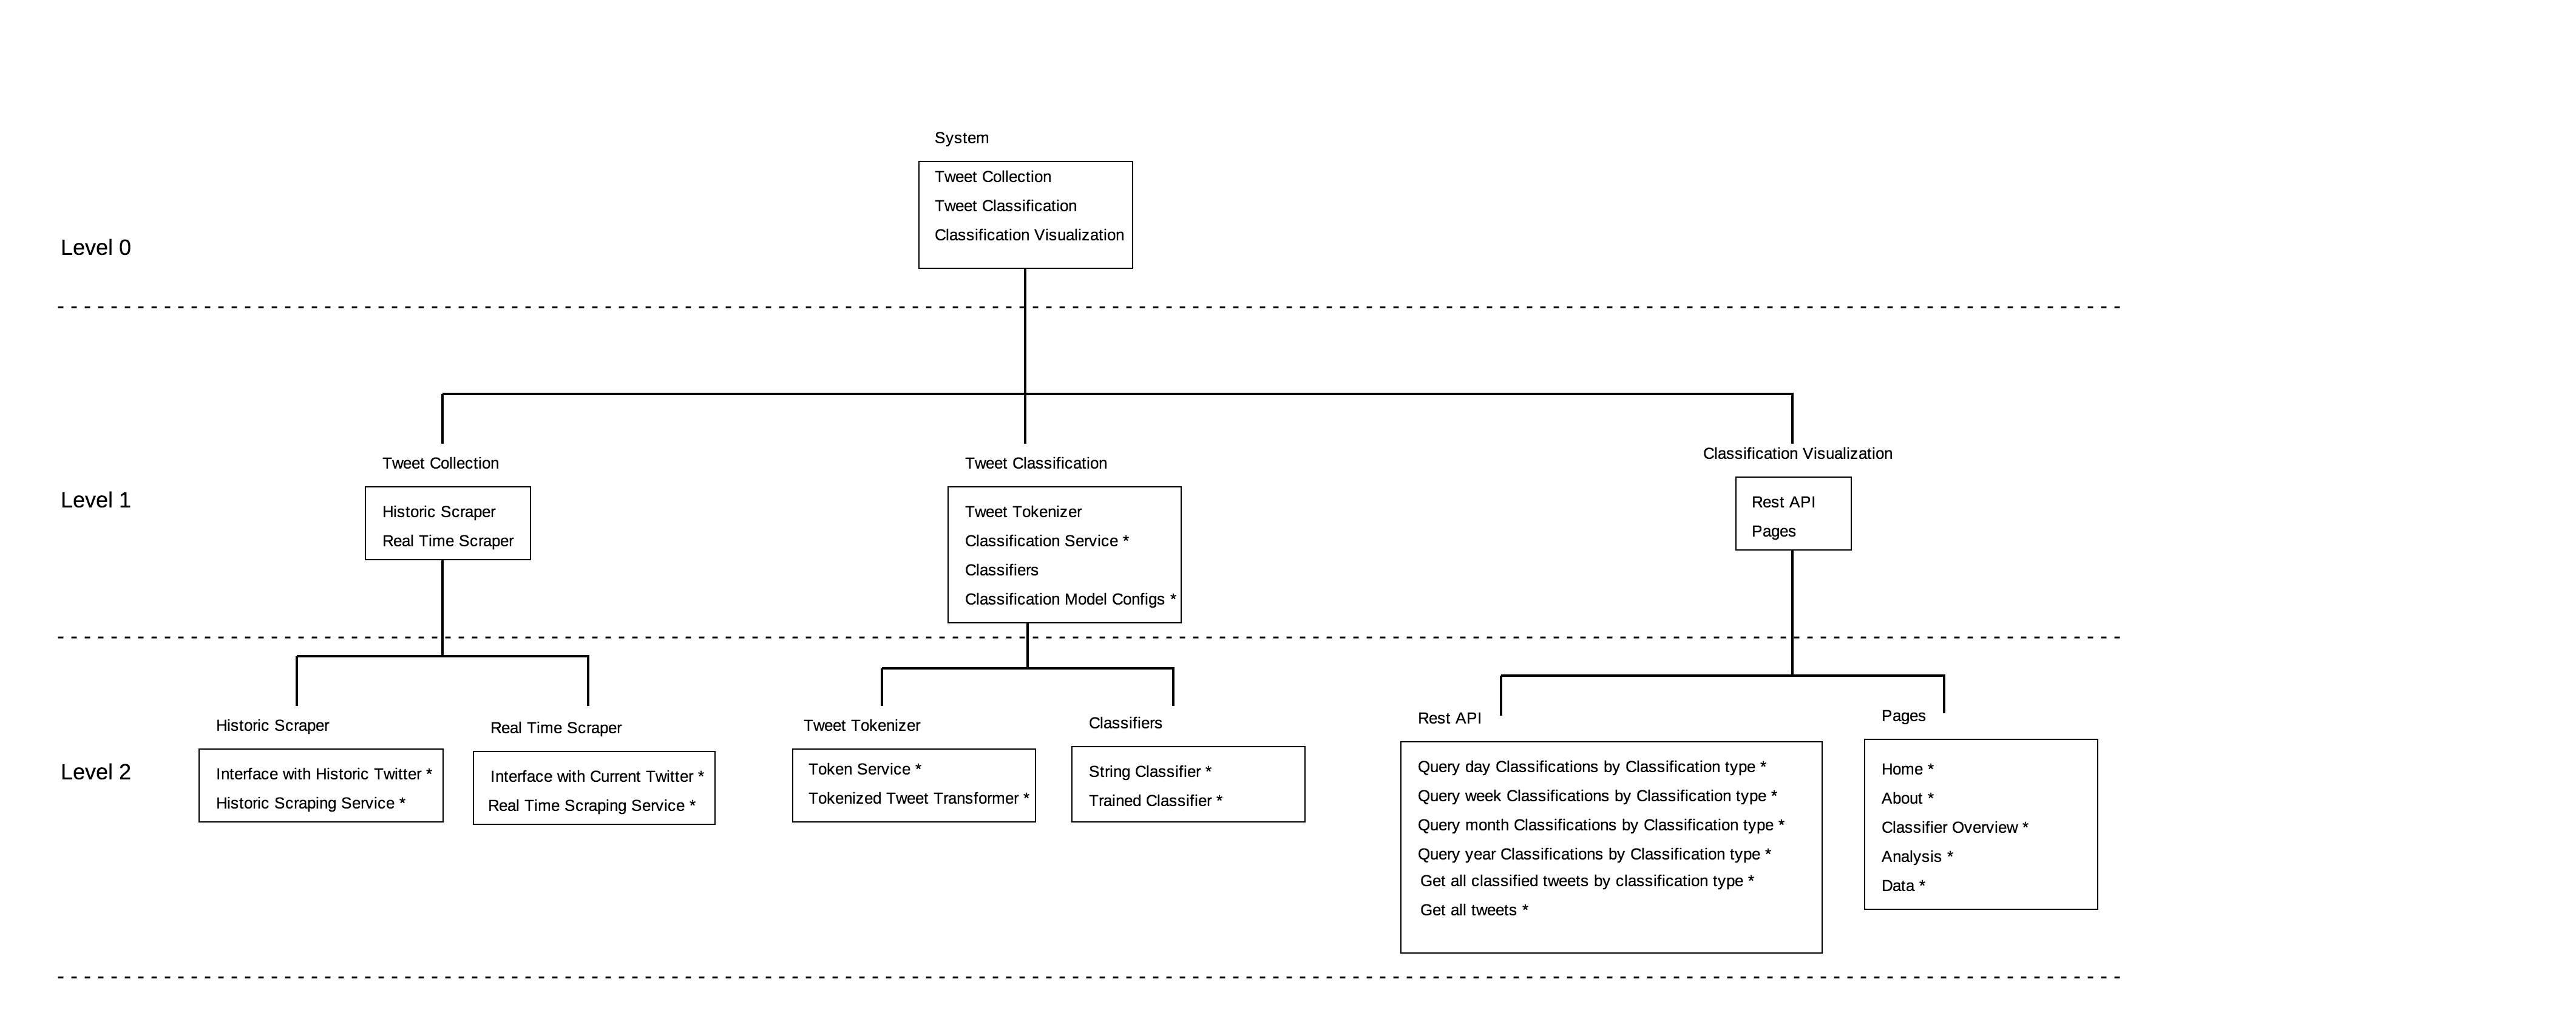
\includegraphics[width=22.5cm,height=12cm]{images/top-down-final.png}
  \captionof{figure}{Top Down Design Approach.}
  \label{fig:top-down}        
\end{landscape}


\begin{landscape}
\begin{center}
  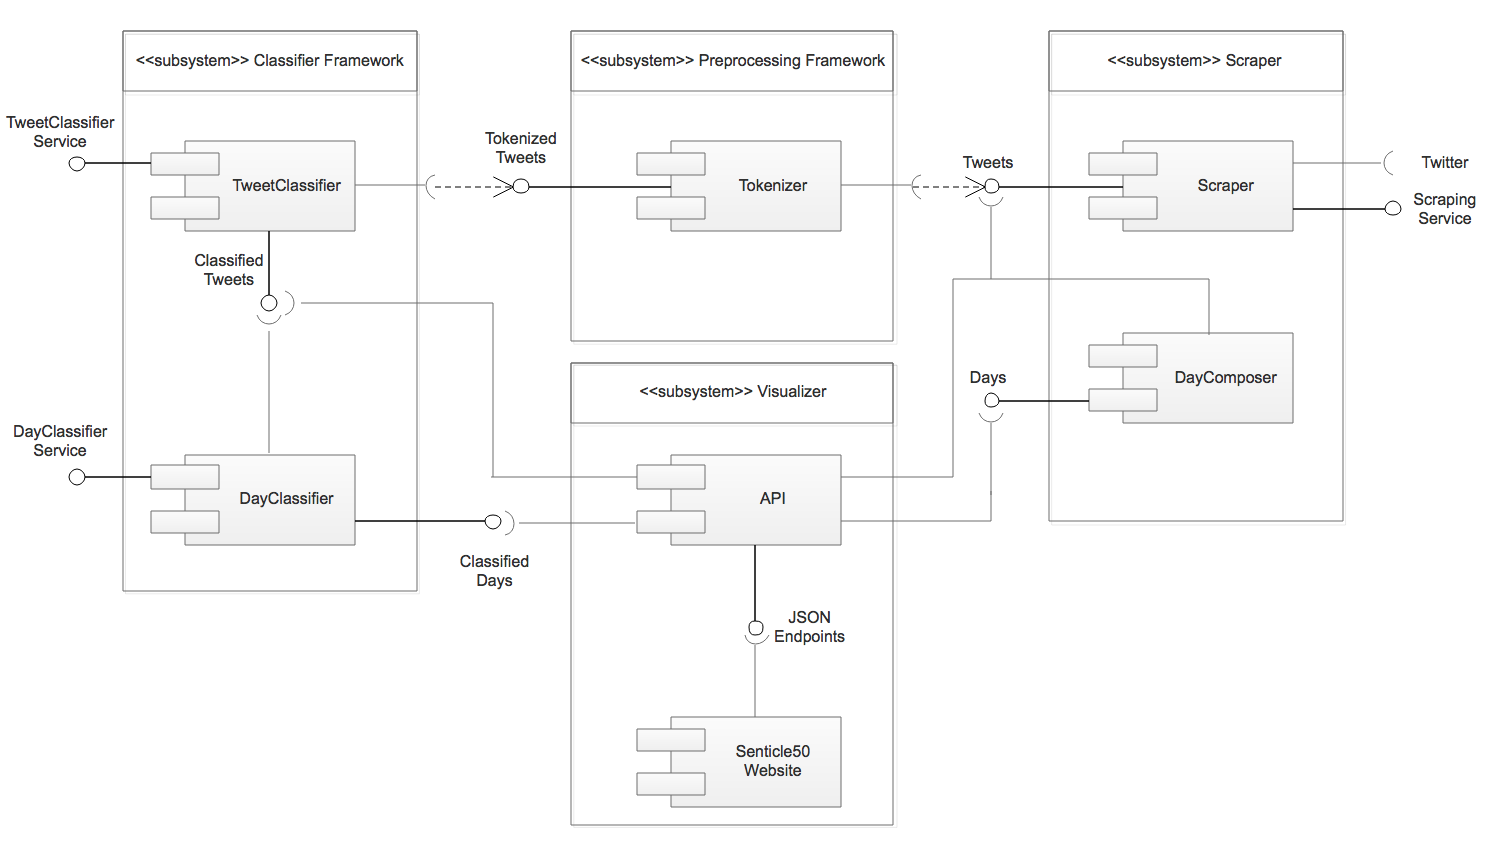
\includegraphics[width=\linewidth]{images/component-diagram.png}
  \captionof{figure}{Component diagram.}
  \label{fig:component}
\end{center}
\end{landscape}

\section{Classifier Architecture}
The System is architected in such a way to split the model from the classifier itself as well as an interface structure which enforces each classifier implements the base required classifier methods. Having this structure allows for a number of beneficial qualities as listed below.

\begin{center}
  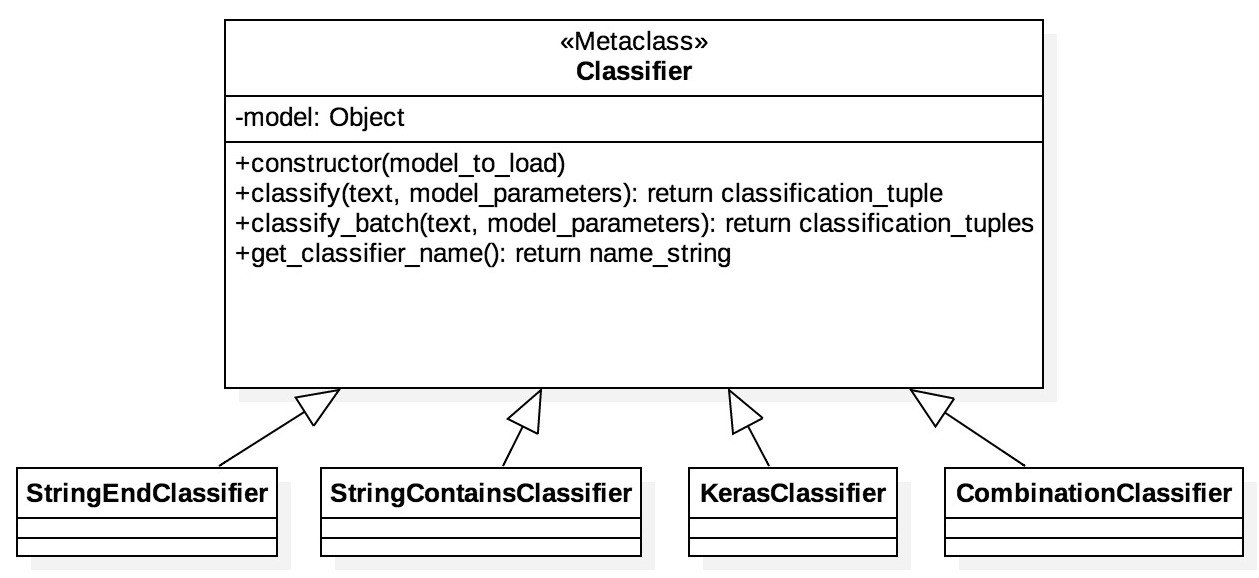
\includegraphics[width=12cm]{images/classifier-inheritance.jpg}
  \captionof{figure}{Classifier Interface Structure.}
  \label{fig:classifier-interface}
\end{center}

\subsection*{Generic Classifiers}
Classifiers are unique to the model type they can serve, the classifier classes are placeholder classes for the model i.e. a model is an attribute of a classifier and thus one classifier class can serve multiple models of the same base model type.

\subsection*{Pluggable Classifiers}
The System structure of multiple classifiers implementing methods from the base classifier object ensures that new class implementations of a classifier can be implemented and plugged into the classification framework at ease.

For a new classifier to be plugged into the framework it must include:
\begin{itemize}
\item a constructor taking the model attribute to classify against.
\item a classify method to classify one tweet.
\item a batch classify method for classifying batches of tweets.
\item a get method to return the classifier name for storage in the classifier registry.
\end{itemize}

\section{Database Schema}
The System as identified in the analysis and specification required a database to permanently store the sentiment analysis that it has computed. The architectural process undertaken to design the database was to first use the analysis of related systems to list data that is expected in this system. After all the data was listed, entities were extracted such as ``Tweet''. Each entity had it's corresponding attributes extracted. 

\subsubsection*{Modelling the Data}
The database now had a preliminary design where each of the entities was representative of the database tables. The entities were first modelled first using a conceptual data model to solidify the relations between each of the tables and the attributes which belonged to each relation. The conceptual model was then converted to a physical model to gain an understanding of the attribute key relations and the types required to model each attribute within a physical database.

\subsubsection*{Normalization}
The list of tables that were modelled using the physical and conceptual models was normalized to Boyce-Codd Normal Form \citep*{CoddRecentInvestigationsRelational1974} to prevent data redundancy and undesired database behaviour i.e. insertion, deletion or update anomalies.
\\

The normalization of the schema required that for each table R within the designed database, BCNF(R) holds true such that for every functional dependency of R i.e. X\textrightarrow Y (where attribute Y depends on the value of X) either of the following conditions must be true;

\begin{itemize}
\item X\textrightarrow Y is a trivial functional dependency ($Y  \subseteq X$) 
\item X is a superkey (set of attributes within a table whose values can be used to identify a unique record) of table R
\end{itemize}

The result of applying BCNF to the preliminary database design was the creation of more tables e.g. the table ``Label'' was extracted out of ``Classified\textunderscore Tweet'' into its own table due to its functional dependency on `\texttt{Classification\textunderscore Type} and not \texttt{Classified\textunderscore Tweet.Id}. The resulting changes to the database were amended within the database models and thus the final conceptual and physical database structure can be viewed by Figure \ref{fig:conceptual-erd} and Figure \ref{fig:physical-erd}.




\newgeometry{a4paper,left=1in,right=1in,top=1in,bottom=1in,nohead}
\begin{landscape} 
\begin{center}
  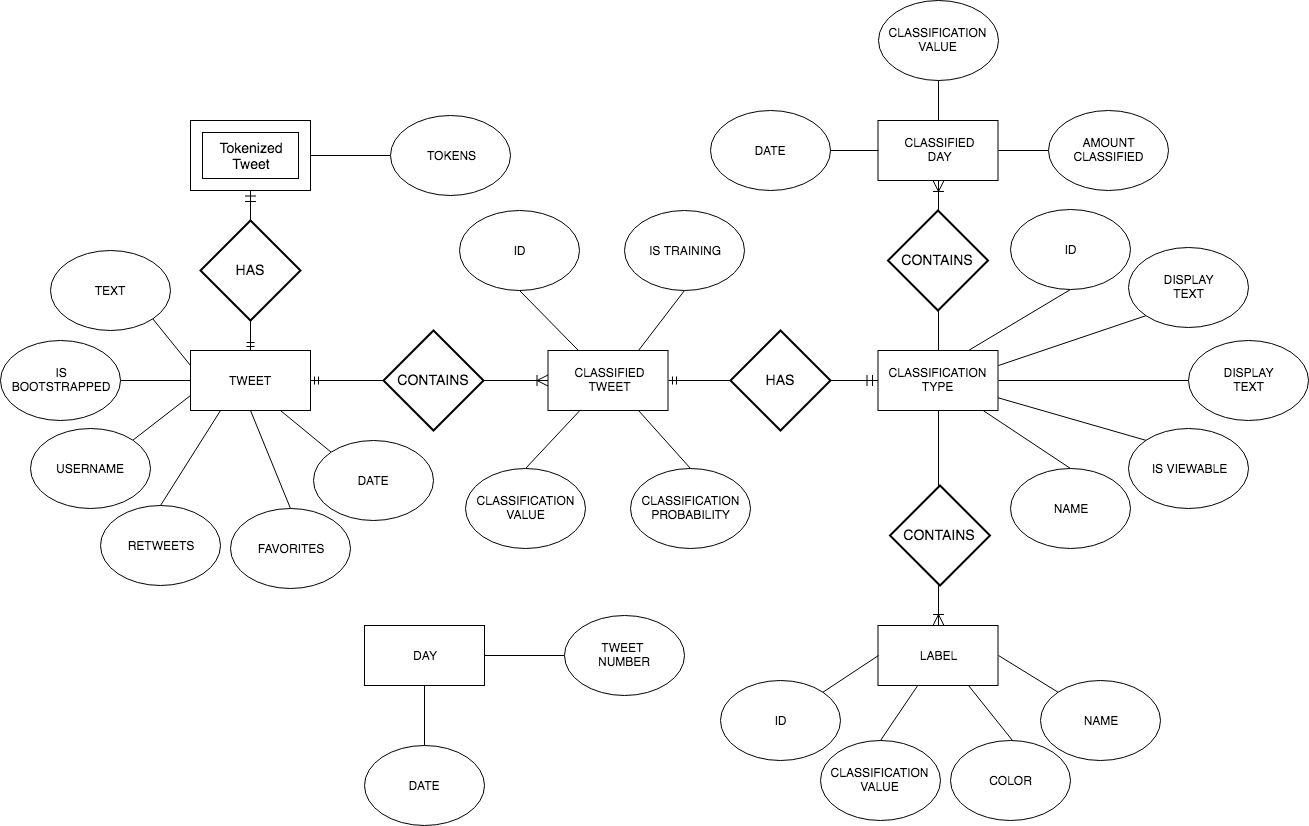
\includegraphics[width=22cm]{images/conceptual-erd.jpg}
  \captionof{figure}{Conceptual Entity-Relationship Diagram.}
  \label{fig:conceptual-erd}
\end{center}
\end{landscape}

\begin{landscape} 
\begin{center}
  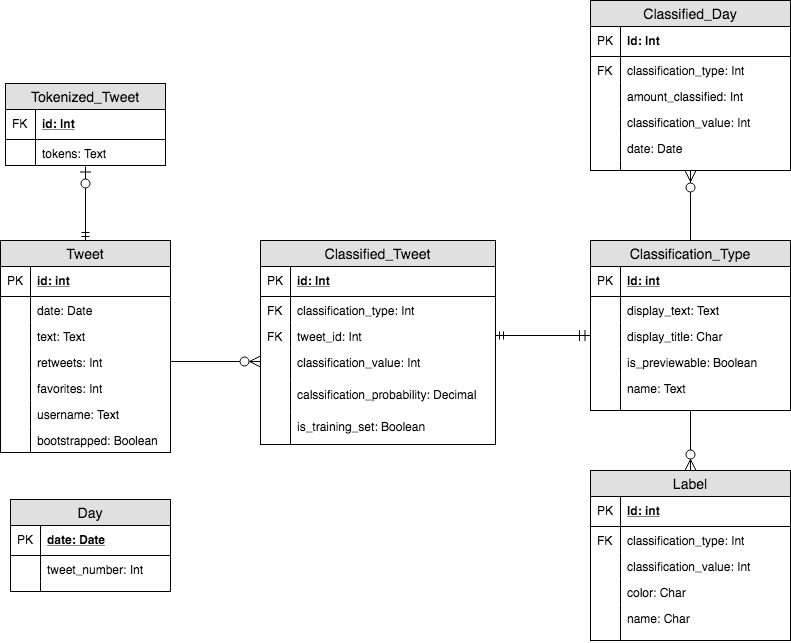
\includegraphics[width=\textwidth]{images/physical-erd.jpg}
  \captionof{figure}{Physical Entity-Relationship Diagram.}
  \label{fig:physical-erd}
\end{center}
\end{landscape}
\restoregeometry % Restore the global document page margins

\clearpage

\section{Design Patterns}

\subsection*{Registry Pattern}
As mentioned each classifier is a separate class and therefore to enable a generic service to decide which Classifier to use when given a configuration file the rationale was taken to design a  \textbf{Classifier Registry} that on-load of the System registers all of the classifiers classes which are available in the System. The registry can then be used to retrieve the class file of a requested Classifier in the system.

\subsection*{Handler Service Transformer Pattern}
For each of the background operations, the system handles the operation request through a handler which calls a service that utilizes a transformer to convert computed attributes into an object form readable by the System.

Each layer in an operation therefore has set responsibilities and can be summarized as follows:

\begin{itemize}
\item Handler: Calls services required with their respective parameters
\item Service:  Encapsulates the business logic and the utilization of a transformer class to convert it's computed attributes
\item Transformer: Converts parameters into a System object.
\end{itemize}

\section{Models}
\subsection{Naive Brexit Stance Model}
The Naive Brexit Stance Model was designed to determine a tweet as having ``Leave'' or ``Remain'' sympathies towards the topic of ``Britain Leaving the European Union''. The model was trained using tweets ending in leave or remain hashtags based off of previous work in the Sheffield System  \citep{maynard_framework_2017}. See Table \ref{table:naive-labels} for the specific class labels from which the classifier learnt natural language patterns unique to the mutually exclusive leave and remain sides of the discussion.
\\

\textit{N.B. It's naivety lies in the absence of using sentiment when classifying a tweets stance
(see Brexit stance for how sentiment can be used to further improve stance detection)}

\clearpage

\begin{center}
\begin{tabular}{ |p{1.5cm}||p{5cm}| }
\hline
 Class & Label\\
 \hline
 Leave &  \#VoteLeave \#LeaveEU\\
 \hline
 Remain &  \#StrongerIn, \#VoteRemain\\
 \hline
\end{tabular}
\captionof{table}{Naive Brexit Model Labelling}
\label{table:naive-labels}
\end{center}

\subsection{Sentiment Model}
The Sentiment Polarity Model was designed to determine a tweet as being ``Positive'' or
``Negative'' sentiment using the textual content of the tweet. The distant labelling technique
chosen for use within this model was the use of distant plain-text emoticon labels i.e. tweets
that contain positive emoticons and no negative emoticons and vice versa (see Table  \ref{table:sentiment-labels} for the specific class labels). Using this distant labelling technique within the training it learnt natural language patterns unique to positive
and negative tweets that aided in classifications.

\begin{center}
\begin{tabular}{ |p{1.5cm}||p{5cm}| }
\hline
 Class & Label\\
 \hline
 Positive & ":)", ":-)", ": )", ":D", "=)"\\
 \hline
 Negative &  ":(", ":-(", ": ("\\
 \hline
\end{tabular}
\captionof{table}{Sentiment Model Labelling}
\label{table:sentiment-labels}
\end{center}

\subsection{Brexit Stance Model}
The Brexit Stance model uses a tweets classifications from the Naive Brexit Stance and
Sentiment models to identify it as having Leave or Remain sympathies.
\\

The model maps the positive sentiment tweets to the Brexit stance it was identified as
(using the Naive Brexit Stance model) and the negative sentiment tweets to the opposite
stance from which it was originally identified as (using the Naive Brexit Stance model).
\\

This classifier therefore acts on the assumption that a tweet that is classified as having
contents regarding one side of the Brexit Debate does not support that side if the sentiment
of the tweet is negative and thus classifies negative tweets to the opposite side from which
it was originally identified.

\clearpage

\section{System Pipeline}
The main high-level operation of visualizing the sentiment analysis of tweets within real time requires that collected tweets pass through the components provided by the System in a chronological order and thus as part of design a System pipeline was conceived. The pipeline is traversed by each tweet collected and can be visualized using Figure \ref{fig:syspipe}.

\begin{center}
  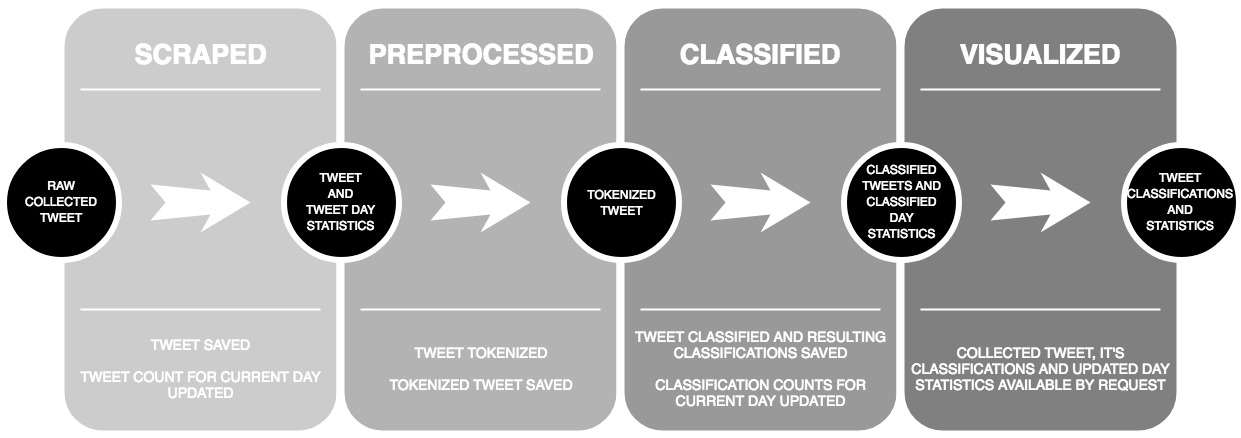
\includegraphics[width=\textwidth]{images/syspipe.jpg}
  \captionof{figure}{System Pipeline.}
  \label{fig:syspipe}
\end{center}

\section{Constraint Resolution}

The project as previously identified in the Specification has a number of limiting/constraint factors that were considered in the design of the system. 

\subsection*{Execution Time} 

\subsubsection*{Concurrent Tasks}
The System within its high-level operations will repeatedly perform the same task on each input i.e. for tokenization each tweet will undergo the same series of tokenization steps. This repetition is an ideal candidate for concurrent activity which fuelled the design behind utilising a thread pool executor to perform tasks in the system which can occur concurrently. The System therefore allows for the specification of worker threads within the system operations that use a thread pool to result in a linear decrease of execution time as thread numbers increase.

\subsubsection*{Asynchronous Tasks}
The System contains actions that are time-consuming to execute and the result of such actions is not needed by the caller of the actions themselves i.e. the saving of items to the database. Having to wait for these operations to occur despite not needing the result can slow down the overall execution of the system. The System combats these tasks by executing them asynchronously in the background allowing for the system to carry on processing and not wait for execution of such tasks.

\subsubsection*{Live Processing}
The System's visual component requires access to tweet count and classification statistics which will be requested via HTTP GET requests. The execution time of calculating statistics such as a sum or maxima grows exponentially with the volume of data on which the statistic is being calculated and as a consequence is unsustainable for serving HTTP requests in a timely manner (on an ever-growing dataset). Therefore the system design incorporates composite objects for statistics which describe the statistics of tweet count and classification count for each classifier on a day granularity. The number of records involved in a statistic calculation is therefore reduced to the number of days in the given time period opposed to the number of tweets. By utilizing composite objects the system execution time for live processing is significantly reduced when serving HTTP requests.

\subsection*{External Storage Size} 
The System will potentially accept up to thousands of tweets per day, it is therefore important that the storage and processing of this data do not occupy too much space. To approach this, the system's relational database schema was designed to be in normalized form and therefore minimize data redundancy by having data records only stored once and related via relations i.e. a tweet is only stored once with a primary key to which related tables use as a foreign key reference. The system also conserves memory by ensuring that only data required by the system is stored i.e. a tweet is stored as a reduced model of the raw input of a tweet (containing only the core details required for the system to operate).

\enlargethispage{\baselineskip}
\enlargethispage{\baselineskip}
\subsection*{Tradeoff Resolution} 

Execution Time vs RAM: The System must strive to be as efficient in time as possible but must beware of the tradeoff with RAM such that operations must be timely but not deplete the system of too much memory resource. To combat this, system features which operate on large amounts of data have been designed to be processed in batches. The Batch processing allows for the system to scale its batch size based on the specifications of the host system it is operating on and thus provides a compromise between Execution Time and RAM that maximizes the efficiency of the system.

\end{document}

\documentclass[11pt]{report}
\usepackage{standalone}
\graphicspath{ {images/} }
\setcounter{tocdepth}{5}
\setcounter{secnumdepth}{5}
\usepackage{natbib}
\usepackage{bibentry}
\bibliographystyle{agsm}
\usepackage{etoolbox}
\setlength{\parindent}{0em}
\setlength{\parskip}{0.25em}
\usepackage[raggedright]{titlesec}
\usepackage{hyperref}
\usepackage{capt-of}
\patchcmd{\bibliography}{\section*}{\section}{}{}
\titlespacing*{\chapter}{0pt}{-40pt}{10pt}
\titleformat{\chapter}[block]{\normalfont\huge\bfseries}{\thechapter}{15pt}{}
\usepackage{rotating}
\usepackage[titletoc]{appendix}
\usepackage{pgfgantt}
\usepackage{graphicx, rotating, caption, lscape, threeparttable}% \usepackage{amsmath}
\usepackage{array}
\usepackage{pdflscape}
\usepackage{geometry}
\usepackage{listings}
\usepackage[T1]{fontenc}
\usepackage[bottom]{footmisc}
\usepackage{subcaption}
\usepackage{float}




\begin{document}
\chapter{Implementation}
\section{Software Stack Selection}

\subsection{Programming Language}
The System as analyzed in the specification requires a number of common computational tasks including web-scraping, natural language processing, machine learning, database interfacing and task execution handlers. To avoid reinventing the wheel within the scope of the system, the design decision of utilizing libraries where possible was taken. Libraries for the above-mentioned operations exist across popular programming languages however through further analysis Python became the obvious candidate. Python as a language promotes the integration of existing Python modules and `has an active supporting community of contributors and users that also make their software available for other Python developers to use under open source license terms'  \footnote{Python Modules accessible via https://docs.python.org/3/installing}.

\subsection{Framework}
The componentized system as highlighted in Figure \ref{fig:component} consists entirely of back-end components except for the singular visualizer front-end component. Due to the API nature of the back-end interfacing with the front-end, there was room to have a complete separation between the back-end and the front-end where a Python back-end would power a front-end framework that is completely detached from the business logic of the back-end system. However, the bulk of the requirements laid in the back-end and thus having a separate framework for the front-end could be argued to be overcomplicating the implementation of what is a well-structured System architecture. The design rationale was therefore taken to implement the back-end and front-end in a singular framework whilst upholding the design of having the business logic and API in the back-end allowing future extensibility of pulling the front-end into a separate framework at a later date if the System required it.
\\

Having decided on a singular framework for the system, the approach was taken to research and compare the top three python frameworks that would offer full stack capabilities along with a number of identified desirable quantities needed in the framework. Using the comparisons conducted in Table \ref{table:framework-comparison} and further research the framework decided upon was Django for it's out of the box capabilities and separate application support being most appropriate for the proposed solution (batteries included).
\\

\begin{tabular}{ |p{1.5cm}||p{2cm}|p{2cm}|p{2cm}|p{1.75cm}|p{1.75cm}|  }
 \hline
 \multicolumn{6}{|c|}{Full Stack Python Web Framework Comparison} \\
 \hline
 Name & Python Version Required & Separate Application Support & Templating & Batteries Included & Github Stars\\
 \hline
 Django & 3.X    & Yes &   Yes & Yes & 32,770\\
 Flask &   $\geq$ 3.3  & No & Yes & No & 34,207\\
 Pyramid & $\geq$ 3.4 & No &  Yes &  No & 2,700\\
 \hline
\end{tabular}
\captionof{table}{Python Framework Comparison \textbf{as of publishing date}}
\label{table:framework-comparison}

\section{System Architecture}
Through the implementation of the Python full-stack framework ``Django'', the system is encapsulated in a set of Python modules separated into ``applications'' that represent the high-level components of the system. Each application is registered within the system and contains a number of Python classes which are responsible for providing the component responsibilities that the application represents. The System also contains utility modules which are used across all the applications and therefore are available at the top level of the system. Along with applications, there are multiple configuration files and scripts that enable the remote execution of the system.

\subsection{Applications}
The applications provided by the system and the component that they represent are as follows:

\begin{itemize}
\item \textbf{classifiers}: representative of the classifier framework component.
\item \textbf{core}: representative of the visualizer component.
\item \textbf{tokenizer}: representative of the preprocessing framework component.
\item \textbf{scraper}: representative of the scraper component.
\end {itemize}

Each application contains a series of classes that provide the functionality required for the application and some Django specific classes for configuration (non-capitalized). If the application interfaces with the database it will contain a ``models.py'' file which are Django representations of the database tables that the application owns. Each application also contains a ``views.py'' file which also forms part of the visualizer component as each applications ``views.py'' file provides API endpoints that populate the template pages when requested.

\subsection{Dependency Injection}
The system contains two methods of dependency injection to provide the system access to third-party libraries of established code, it utilizes a python virtual environment to inject python libraries into the system for use within the back-end components of the system and nodejs is used to inject javascript and CSS libraries into the system for using within the front-end visualizer component of the system. On starting the system, the dependencies are copied over to the global ``static/'' folder from which they are globally accessible from within the system. The configuration files for dependency injection are \texttt{requirements.txt} (back-end injection) and \texttt{package.json} (front-end injection) which both contain a list of dependencies and there versions utilized by the system.
\\

\textit{N.B. Third party libraries that have been used without dependency injection have been clearly stated within the code using a header comment.}

\section{Database Implementation}
The System contains two database implementations, the live production PostgreSQL database hosted via AWS and the auxiliary test SQLite database used for integration testing of the system. The implementation of database structure required the translation of each model in the entity relationship diagrams into Django Models such that the System could then utilize the built-in object-relational mapping (ORM) tool to easily access database records without the need for SQL. Django handles the database management of the system with changes to the models occurring through \textit{South Migrations} which are then propagated to the database. The entities from the physical entity-relationship diagram were translated into Django Models with each attribute from the entity being a field of the representative Django Model. Through translation of the data models, a number of constraints were also implemented to enforce the data integrity within the database. For illustration purposes the translation of the Tweet entity can be seen in Figure \ref{fig:model-translation}

\begin{center}
  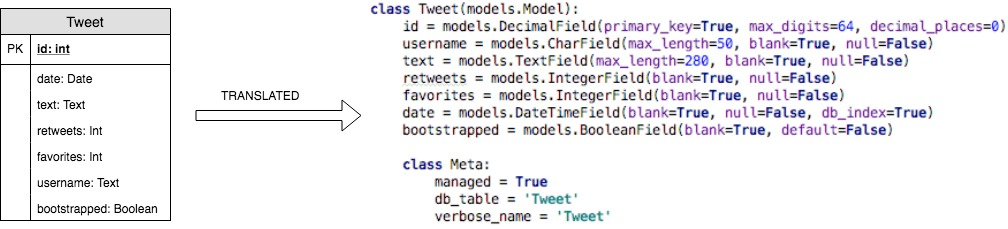
\includegraphics[width=16cm]{images/model-translation.jpg}
  \captionof{figure}{Data Model Translation.}
  \label{fig:model-translation}
\end{center}
\clearpage

\section{System Features}
The System features that were outlined in the proposed specification have their implementations listed below.

\subsection*{Tweet Collection}
The scraper application hosts two interfaces with Twitter for the collection of tweets. Having two application product interfaces (that communicate with Twitter) for the collection of tweets allows for the collection of \textbf{historic} and \textbf{current (in real-time)} tweets.

\subsubsection*{Historic Scraper}
The system integrates the existing third party tweet collector named ``GetOldTweets-python'' \footnote{GetOldTweets-python accessible via https://github.com/Jefferson-Henrique/GetOldTweets-python} that allows for the backdating of tweets older than two weeks. It does this by manually scraping the JSON of the twitter advanced search timeline using the requested dates, languages and hashtags as filter criteria. The historic interface was amended to work within the Django framework and optimized using the system's concurrency utilities to allow for thread pool execution of the extraction of tweets from the JSON as well as asynchronous saving of tweet objects to the database.

\subsubsection*{Real Time Scraper}
The system integrates the existing third party tweet collector named ``Tweepy'' \footnote{Tweepy accessible via http://www.tweepy.org/} that allows for the collection of tweets in real time i.e. as they are posted. Tweepy allows the system to communicate with twitters firehose (tweet access) provider ``gnip'' and request access to real time tweets for a specified language and hashtags.
\\

Tweepy enables a connection between the client application and gnip to be established, then queries the streaming API with the filter criteria resulting in the delivery of tweets to the client application as they are posted and upon close of the connection attempts to retry connecting until a new connection is established and the collection restarts. The raw tweet JSON objects are placed in a Redis message broker to process the saving of tweets asynchronously via a celery application. The asynchronous processing is key to the operating of real-time collection as gnip delivers tweets from a fixed size queue which only holds tweets for a limited time before disposing of them. Celery (an asynchronous task executor) then processes the receive tweet task in which the raw tweet JSON is converted into a tweet model object and then saved to the database.

\begin{center}
  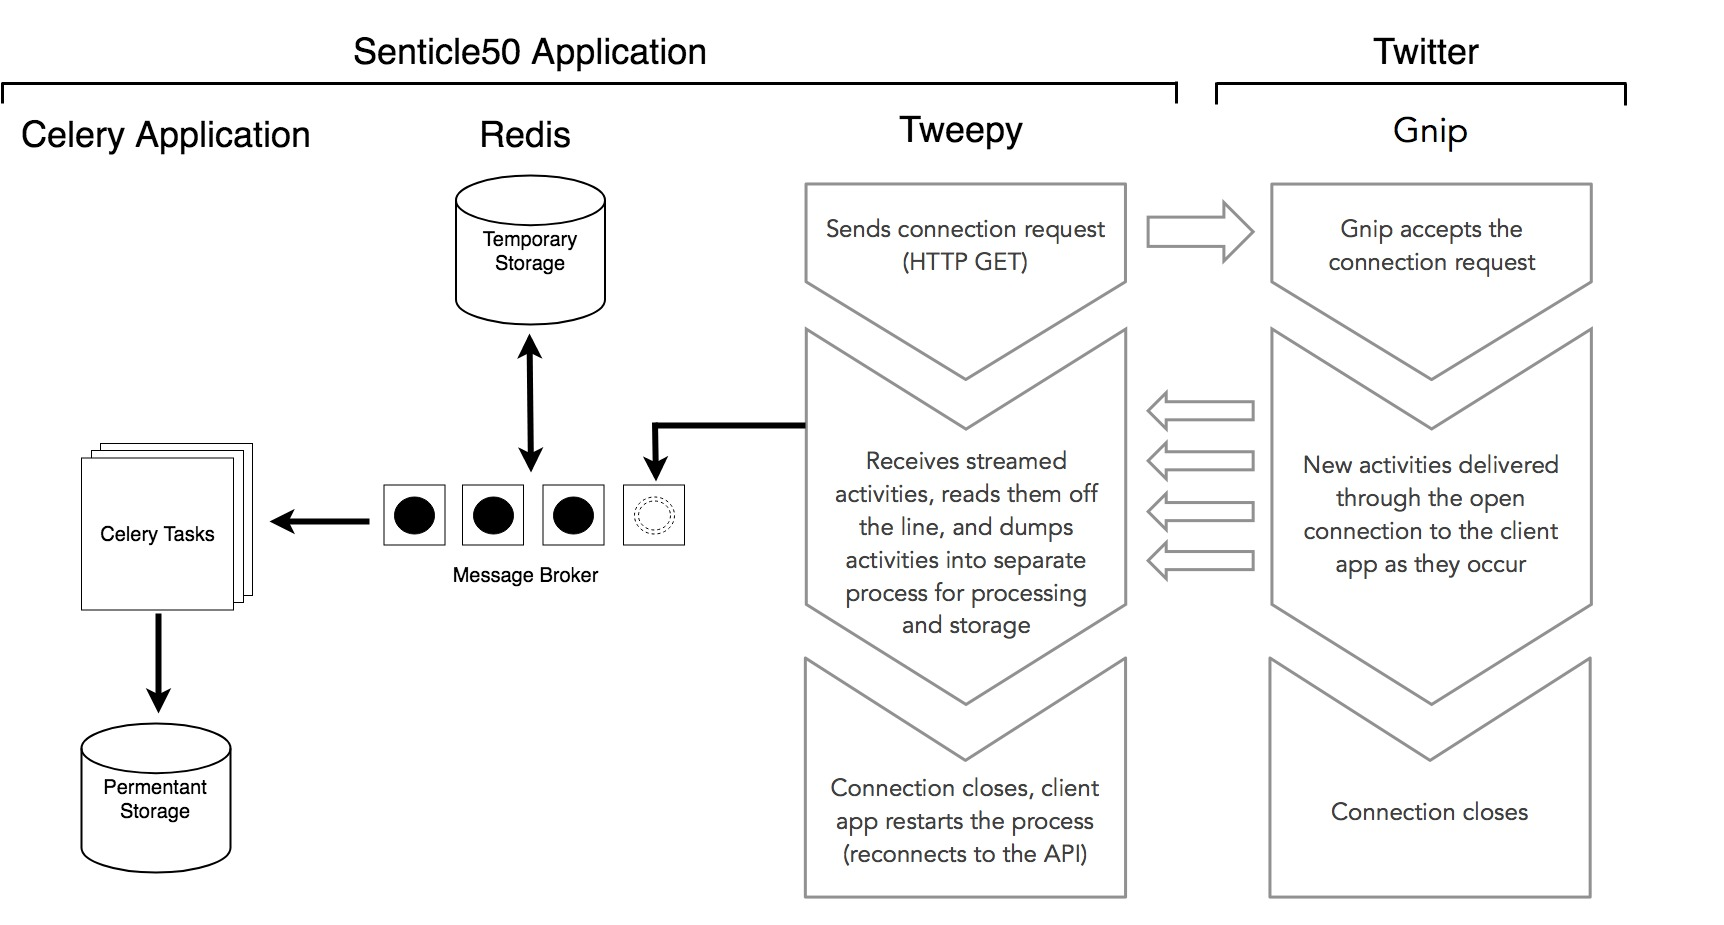
\includegraphics[width=\textwidth]{images/real-time-tweet-collection.jpg}
  \captionof{figure}{Real-Time Tweet Collection \protect\footnotemark.}
  \label{fig:syspipe}
\end{center}

\footnotetext{Modified Image accessible via http://support.gnip.com/articles/consuming-streaming-data.html}

\subsection*{Tweet Tokenization}
The tokenizer application implements the preprocessing step of tweet classification, it manipulates the raw text of tweet objects and converts tweets into a ``Tokenized Form''.
\\

Each Tweet is converted into a string of ``Tokens'' through a series of tokenization steps that utilize regular expressions and the natural language toolkit to accomplish this. A tweet's raw text will therefore go through the following steps in order

\begin{enumerate}
\item All text is lowered in case.
\item Twitter Mentions are replaced e.g. @UserMention.
\item Hashtags are removed e.g. \#Example.
\item Twitter ``RT'' symbol for retweet is removed.
\item Extra whitespace is removed
\item URL's are removed e.g. http://url.com
\item Stop words are removed e.g. his/her.
\item Punctuation is removed e.g. ! , / ' ( )
\item Remaining text is split into an array of tokens (words)
\item Words are stemmed to reduce dimensionality of feature set e.g. running -> run
\item Final tokens are joined back together as a token string.
\end{enumerate}

\subsection*{Tweet Classification}

The classifiers application implements the classification framework component of the system. The set of implemented classifier classes contains the  \texttt{CombinationClassifier}, \texttt{KerasClassifier}, \texttt{StringContainsClassifier} and \texttt{StringEndClassifier}. Each of the the implemented classifiers classifies tweets against a model which is passed in as an attribute when instantiating the classifiers as mentioned in the Design. The classifiers application exposes two main services that can be interacted with, the \texttt{ClassifierService} for classifying tweets on a one tweet per classification basis and the \texttt{BatchClassifierService} for classifying larger groups of tweets on a batch basis. The classifiers application also provides two registry classes that implement the registry pattern discussed in the design; the \texttt{ClassifierRegistry} and \texttt{RealTimeClassifierRegistry}.

\subsubsection*{Model Architecture}
The models that utilize a neural network i.e. the \texttt{Naive Brexit Model} and \texttt{Sentiment Model} have been created using the Neural Network library Keras. Each of the models convert the tokenized tweets into a padded vector of 140 length (that can represent the new max length of 280 characters within tweets). Each entry in the vector therefore represents the presence of a word using the index of the word from the tokenized feature set of the top five thousand words found in the training set of the model. Utilizing this structure in the model therefore takes the context (order) of the words as well as the presence of the words for learning patterns of order unique to the classes through the convolutional layers defined within the network. See the experiments application \texttt{management/commands/} folder for the model neural network structures.

\subsubsection*{Classifier Architecture}
The architecture of classifiers has each of the classifiers implement the interface of a Classifier superclass. The set of implemented classifiers within the classifiers application are all subclasses of the abstract base class \texttt{Classifier}. Through the subclass relationship they are required to implement the abstract methods defined within ``Classifier'' and thus the interface relationship is enforced (See Listing .

\clearpage
\begin{center}
\begin{lstlisting}
from abc import ABC, abstractmethod

class Classifier(ABC):

    @abstractmethod
    def __init__(self, model_to_load):
        pass

    @abstractmethod
    def classify(self, text, model_parameters):
        pass

    @abstractmethod
    def classify_batch(self, texts, model_parameters):
        pass

    @abstractmethod
    def get_classifier_name(self):
        pass
        
@classifier
class KerasClassifier(Classifier):

    def __init__(self, model_to_load):
        ...

    def classify(self, text, model_parameters):
        ...

    def classify_batch(self, texts, model_parameters):
        ...

    def get_classifier_name(self):
        ...

\end{lstlisting}
\captionof{lstlisting}{An example of Classifier interface utilization.}
\end{center}

\clearpage

\subsubsection*{Classifier Registries}
The aforementioned classifier registries are populated by the scripts \texttt{RegisterClassifiers} and \texttt{RegisterRealTimeClassifiers} located in the scripts folder within the system wide configuration folder of \texttt{brexit/brexit/}. Each registry is an instantiation of a \texttt{Singleton} base class thus providing system wide access to the available classifiers after being populated on startup of the system.

\begin{center}
\begin{lstlisting}
class ClassifierRegistry(Singleton):
 
    def _init(self):
        self.classifiers = {}

    def get_registered_classifiers(self):
        return self.classifiers

    def add(self, classifier_name, classifier):
        if classifier_name not in self.classifiers:
            self.classifiers[classifier_name] = classifier

    def get(self, classifier_name):
        if classifier_name in self.classifiers:
            return self.classifiers[classifier_name]

        raise ValueError(`Classifier not found in classifier registry')
\end{lstlisting}
\captionof{lstlisting}{ClassifierRegistry.py class implementation}
\end{center}

The ClassifierRegistry provided by the classifiers application allows for a service to be generic by dynamically pulling the class implementation of the configured classifier and instantiating it. 

\begin{center}
\begin{lstlisting}
classifier = ClassifierRegistry().get(config['classifier_name'])
\end{lstlisting}
\captionof{lstlisting}{Usage of ClassifierRegistry}
\end{center}

The \texttt{RegisterClassifiers} script is executed first and populates the \texttt{ClassifierRegistry} with each of the available classifiers within the system that end in ``Classifier''. For a classifier to be registered within the \texttt{ClassifierRegistry} it is required to have the \textit{classifier decorator} which allows for the classifier to be added to registry upon import.

\begin{center}
\begin{lstlisting}
def classifier(cls):
    classifier_registry = ClassifierRegistry()
    classifier_registry.add(cls.get_classifier_name(), cls)
    return cls
    
@classifier
class KerasClassifier(Classifier):
    ...
    @staticmethod
    def get_classifier_name():
        return "KerasClassifier"

\end{lstlisting}
\captionof{lstlisting}{Usage of  ``classifier'' decorator}
\end{center}

After the \texttt{ClassifierRegistry} is populated the \texttt{RegisterRealTimeClassifiers} script begins to populate the \texttt{RealTimeClassifierRegistry} with the json classification configuration files that contain the boolean flag ``is\textunderscore real \textunderscore time'' that is true. It is the configuration files that are contained in the \texttt{RealTimeClassifierRegistry} that are utilized in the real time classification of tweets.

\subsection*{Visualisation}
The application core and the \texttt{views.py} files contained in the rest of the applications together make up the visualizer component of the system. The visualizer component as highlighted in Design is split into pages, with each page begin reachable by the navigation bar (visible at the top of the page) except for the classifier-analysis page which is accessed via buttons within the analysis page and thus is the only second depth page in the visual system. The visual component utilizes bootstrap for css conformity and cross browser/device layout support, jQuery for user interactions and D3 for the analysis pictorial visualisations displayed on the classifier-analysis page. 

\subsubsection*{API}
The system has a number of configured url paths which are registered in the system within \texttt{urls.py} files. These url paths are regular expressions that match the url of a given request and handle the execution of that url accordingly. If the url does not match any of the registered url paths within the system Django returns a page-not-found exception (HTTP 404) and renders the 404.html page found within the \texttt{templates/} folder. On the successful match of a url a \texttt{views.py} endpoint is called to render a template and JSON context that holds the data for the template to display.

\subsubsection*{Template Pages}
The System uses Django's built-in templating feature to populate pages where the information is displayed dynamically i.e. data displayed on the page is not static. The templating structure consists of a base template \texttt{index.html} that defines the overall layout of the website and includes the elements of the site which are viewable regardless of page e.g. navigation header and footer. The base template defines a body section which each child template page then extends with the content of that page. Each template page serves one url except the classifier-analysis page which serves four url's; one for each displayable time unit. Using a single template for the classifier-analysis page allows the rendering of four unique views of the page each of which has dynamic data populated through various permutations of the parameters classifier type and time period.
\\

The final set of viewable implemented pages as outlined in the Design are as follows; \texttt{home.html}, \texttt{analysis.html}, \texttt{classifier-analysis.html}, \texttt{data.html} and \texttt{about.html}.

\begin{figure}[H]
        \begin{subfigure}[b]{0.30\textwidth}
                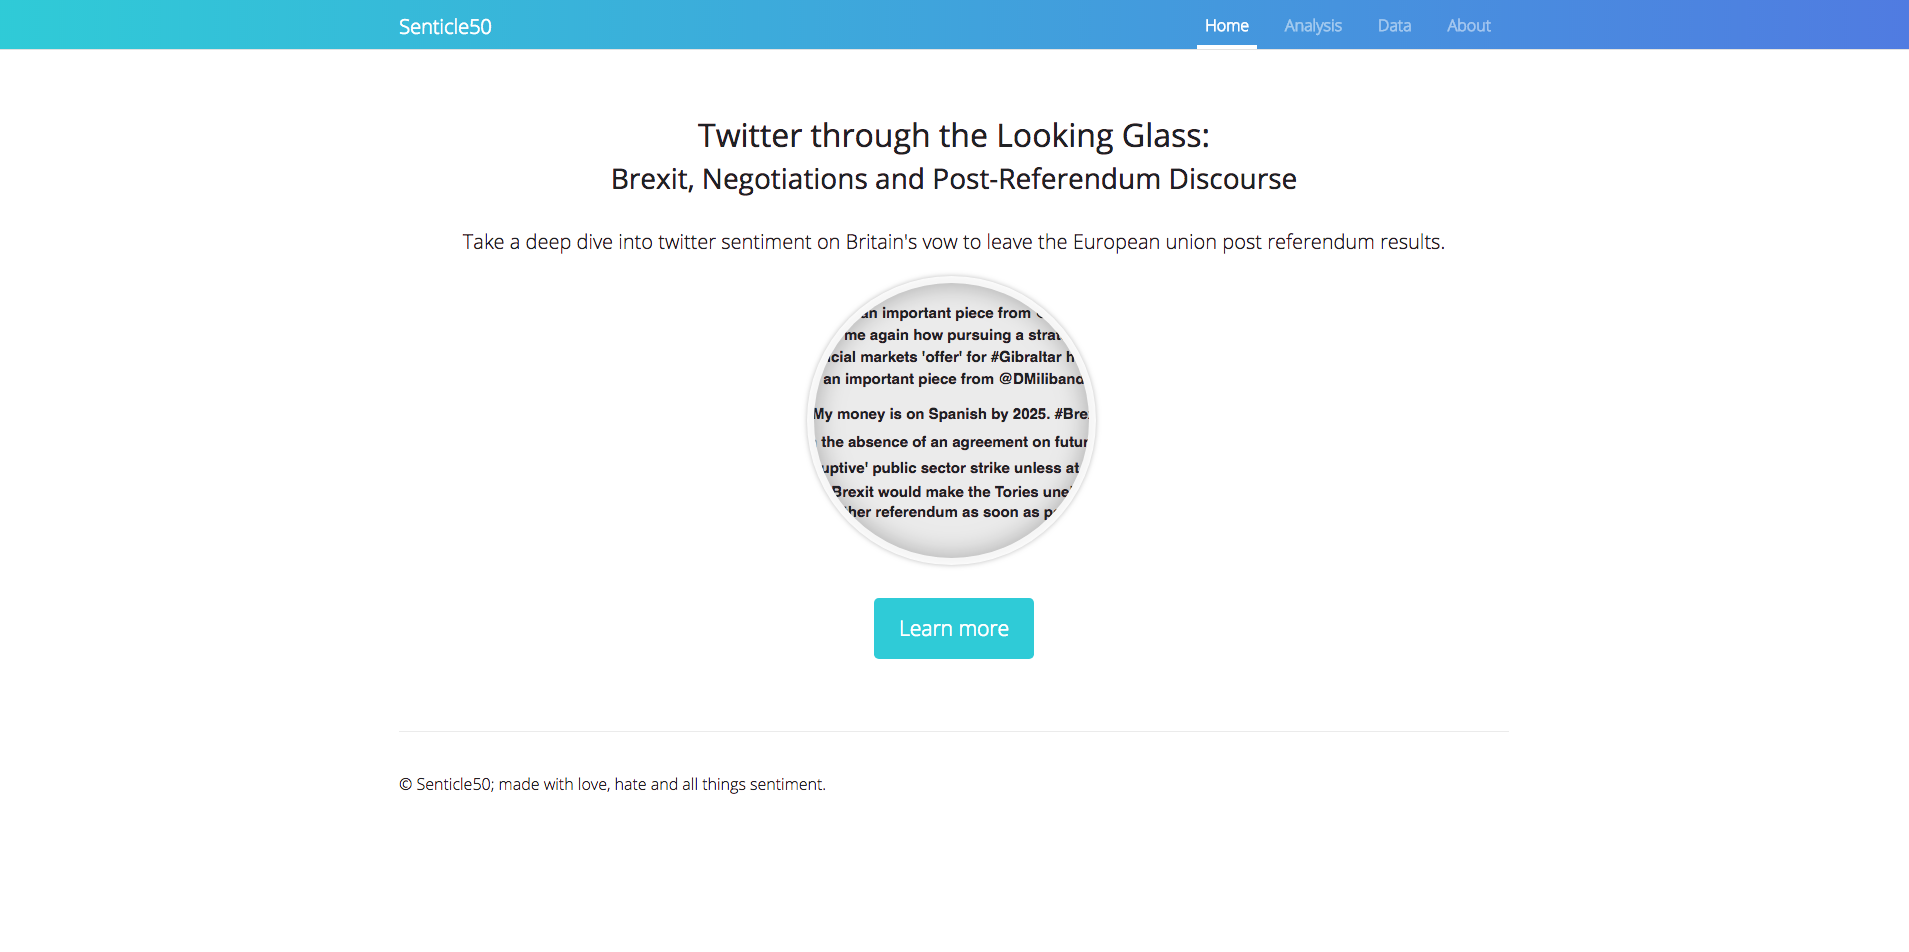
\includegraphics[width=\linewidth, height = 3cm]{images/home.png}
                \caption{home page}
                \label{fig:gull}
        \end{subfigure}%
        \hfill
        \begin{subfigure}[b]{0.30\textwidth}
                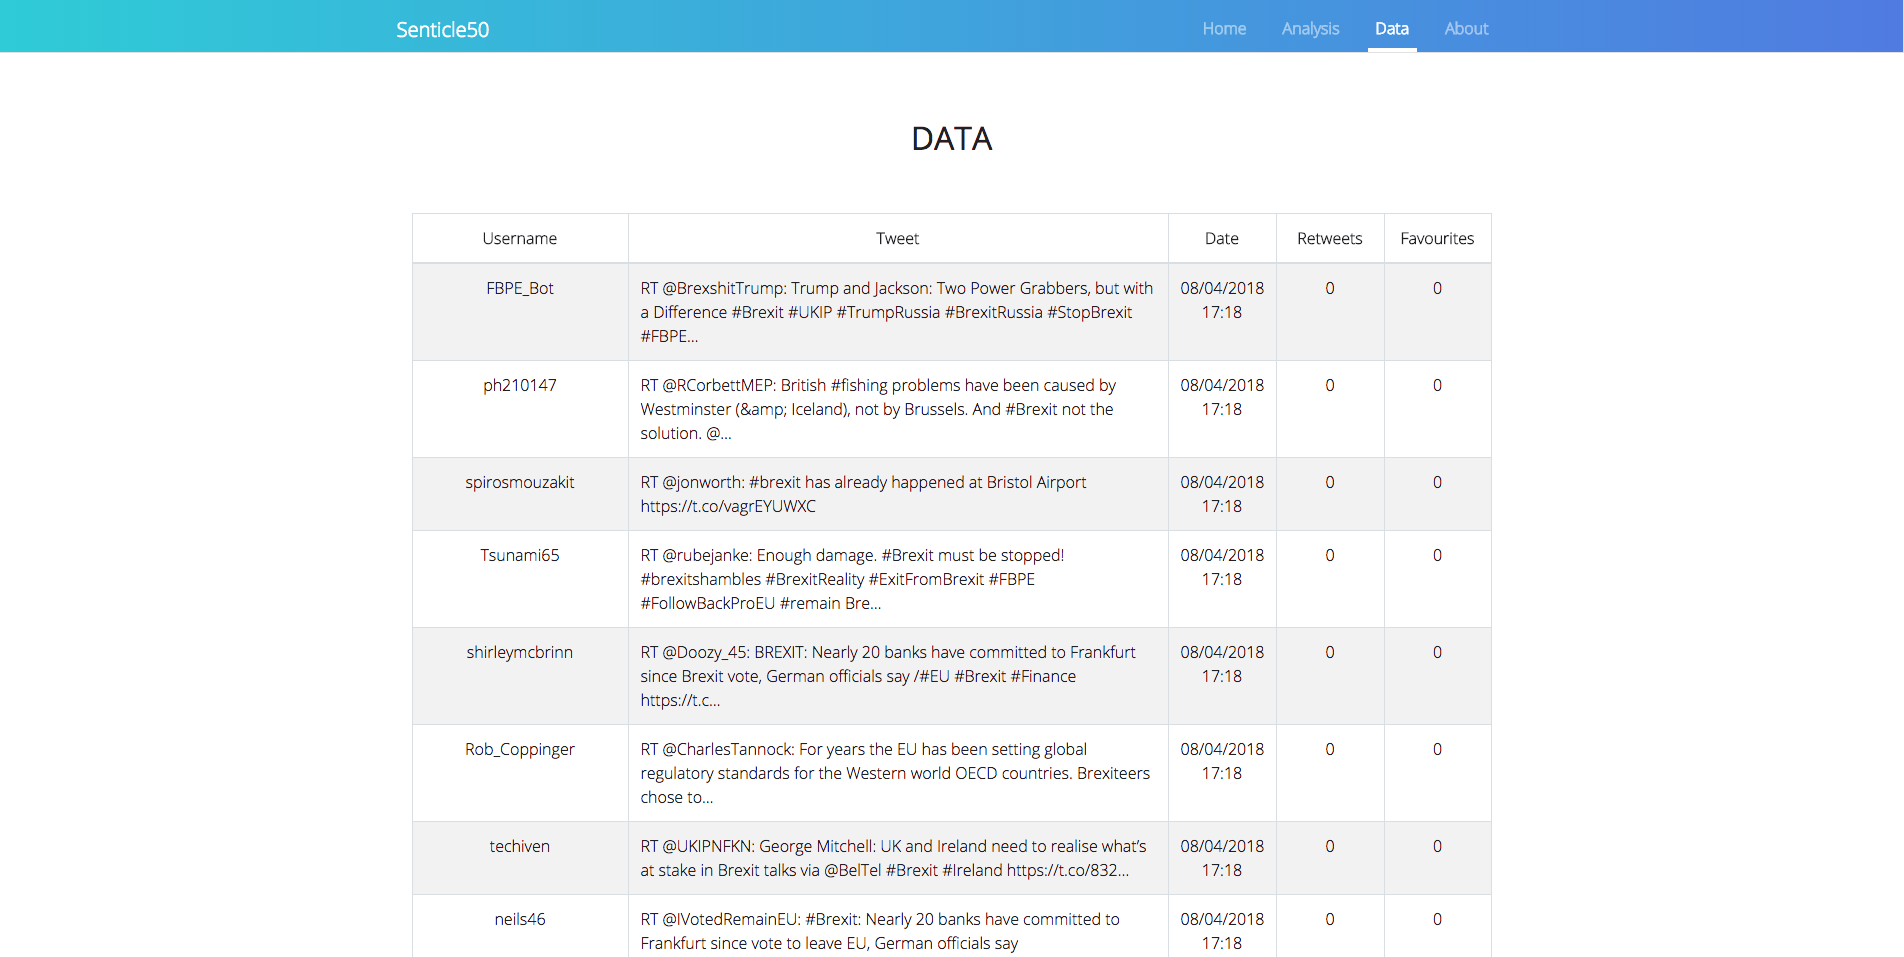
\includegraphics[width=\linewidth, height = 3cm]{images/data.png}
                \caption{data page}
                \label{fig:gull2}
        \end{subfigure}%
        \hfill
        \begin{subfigure}[b]{0.30\textwidth}
                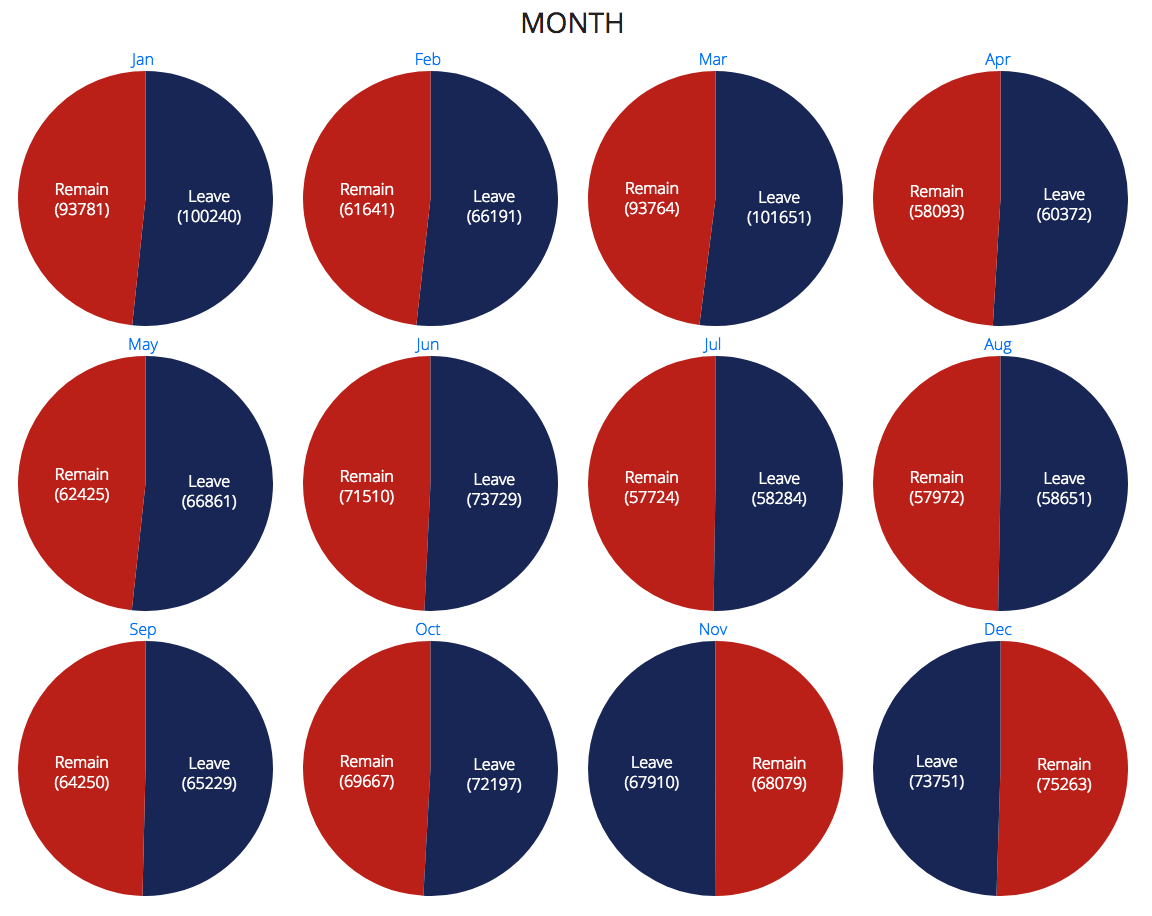
\includegraphics[width=\linewidth, height = 3cm]{images/analysis.png}
                \caption{analysis}
                \label{fig:tiger}
        \end{subfigure}%

        \caption{System Website Screenshots.}\label{fig:screenshots}
\end{figure}

\subsection*{Automation}
The automation of the system is the flow between all of the components within the system. The System pipeline outlined in the Design has been implemented through a series of scripts  that configured remotely on the server. The remote server uses a process control system named Supervisor to ensure all of the automated tasks are running. The system also uses a scheduled cron job to classify the new tweets it has received every five minutes.
\\

The system automation is split into two tasks: the collection and tokenization of a tweet as well as the classification and visualisation of those tweets. As mentioned in the tweet collection system feature implementation, asynchronous tasks are used to convert the real-time collected tweets into tweet models. After conversion to a tweet model the tweet is also tokenized. The collection and tokenization of the tweets requires the running of the system  and the Celery (asynchronous executor) application. To ensure both of these system's are running a Supervisor configuration was enabled for each of commands to run the two systems required. It was found that the classification of tweets on a one tweet per classification basis was inefficient for real time classification as Keras required a lock when asked to predict a class given a sample, hence batch classification and visualisation was chosen to be a task of it's own. The batch classification and visualisation classifies and updates the composite visual objects required for visualisation on the tweets which haven't yet been classified today, this task runs every five minutes on a scheduled cron job.


\enlargethispage{\baselineskip}
\section{Deployment}
\label{sec:deployment}
For the deployment of the system onto the remote virtual private server the continuous delivery environment \textit{Jenkins} was used. Jenkins as a tool allows for the automation of tasks through the specification of a delivery pipeline. The System utilizes a \texttt{JenkinsFile} which specifies the continuous delivery pipeline consisting of a Build, Test and Deploy step (see Figure \ref{figure:deliverypipe}). Upon running the System's pipeline, Jenkins handles the pulling of the System's GitLab repository itself after which it is the Build and Deploy steps of the delivery pipeline which is required for deployment of the System via Jenkins. The Build step first installs a clean environment for the System to run in ensuring that all dependencies are injected, the static front-end files are generated and that the System can be built i.e. that it compiles. After a successful build the Deploy step handles across a secured ssh connection to the remote server; the removal of the old system, the copying of the new system files via the secure copy protocol and the restarting of the system through supervisor commands. Upon successful execution of the delivery pipeline the System is backup within seconds containing the new changes which had been committed to the System's GitLab repository prior to running the delivery pipeline. 
\\

\textit{N.B. If any steps within the delivery pipeline fail, the deployment of the system is aborted with Jenkins displaying the source of error thus preventing a faulty system from being deployed onto the live production server}.

\begin{center}
  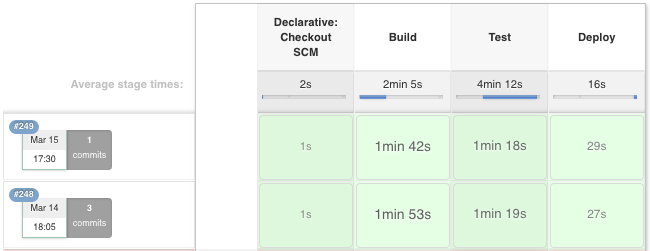
\includegraphics[width=0.9\textwidth]{images/delivery-pipeline.png}
  \captionof{figure}{Jenkins view of the Continuous Delivery Pipeline.}
  \label{figure:deliverypipe}
\end{center}

\end{document}

\documentclass[11pt]{report}
\usepackage{standalone}
\graphicspath{ {images/} }
\setcounter{tocdepth}{5}
\setcounter{secnumdepth}{5}
\usepackage{natbib}
\bibliographystyle{agsm}
\usepackage{etoolbox}
\setlength{\parindent}{0em}
\setlength{\parskip}{0.25em}
\usepackage[raggedright]{titlesec}
\usepackage{hyperref}
\usepackage{capt-of}
\patchcmd{\bibliography}{\section*}{\section}{}{}
\titlespacing*{\chapter}{0pt}{-40pt}{10pt}
\titleformat{\chapter}[block]{\normalfont\huge\bfseries}{\thechapter}{15pt}{}
\usepackage{rotating}
\usepackage[titletoc]{appendix}
\usepackage{pgfgantt}
\usepackage{graphicx, rotating, caption, lscape, threeparttable}% \usepackage{amsmath}
\usepackage{array}
\usepackage{pdflscape}
\usepackage{geometry}
\usepackage{listings}
\usepackage[T1]{fontenc}
\usepackage[norsk,nameinlink]{cleveref}
\usepackage{multirow}



\begin{document}
\chapter{Experiments and Testing}

The designed and implemented system was practically applied to the semantic classification of the tweets regarding the discussion of  ``Britain Leaving the European Union''.
\\

\section{Tweet Collection Experiment}
Previous system's as stated in the related work used a set group of seed hashtags for which they collected tweets for and used as distant labels in their classification models. Instead of manually choosing the seed hashtags like previous Systems the experimentation choice was taken to extrapolate a seed hashtag set to use for collection and distant labelling. Initially, tweets containing either \#Brexit, \#VoteLeave and \#VoteRemain were collected. After collecting tweets from the day of referendum (23/06/2016) up until the initiation of the Brexit negotiations (18/06/2017), the Jacquard's Distance Function (see Figure \ref{fig:distance}) was applied on each of the hashtags found within the tweets to compare the similarity of each of the tweets containing the hashtags discovered and the tweets containing seed hashtags. The result was \textbf{similar\textunderscore hashtags.csv}; an ordered matrix of discovered hashtags that were similar to one or more of the seed hashtags. From the resulting similar  matrix, a bigger seed hashtag set was chosen (see Figure \ref{fig:seed}) whilst manually ignoring anomalous hashtags which were outliers and not on the discussion topic. 

\begin{center}
\[\forall x. \:\: \forall y. \:\: d_J(x, y)=1 - J(x,y) = 1 - \frac{|x \cap y|}{|x \cup y|}\ = 1 - \frac{|x \cap y|}{|x| + |y| - |x \cap y|}\]
\[where\:x = Set(tweets\:containing\:a\:unique\:discovered\:hashtag),\] 
\[y = Set(tweets\:containing\:a\:seed\:hashtag)\] 
\[and\:d_J(x, y) = Jacquard\:Distance\:Function\]
\captionof{figure}{Jacquard Distance Formula Function.}
\label{fig:distance}
\end{center}
\vspace{0.5cm}

\begin{center}
\#BREXIT \#ARTICLE50 \#BREXITDEBATE
                    \#BREXITMEANSBREXIT \#EUREFERENDUM \#EUREF
                    \#VOTELEAVE \#BREXITEER \#IVOTEDLEAVE \#LEAVEEU
                  \#TAKEBACKCONTROL \#VOTEOUT
				\#STRONGERIN \#REMAIN \#REMOANER \#REMAININEU
                  \#VOTEREMAIN \#STRONGERTOGETHER
\captionof{figure}{Generated Seed Hashtag Set.}
\label{fig:seed}
\end{center}
\clearpage

\section{Testing Methodologies}
The goal of testing within the System was to develop an effective test suite to verify and automate the testing of System behaviour. Tests were written for new functionality as the System functionality was developed, and thus the test methodology of Regression Testing was employed to ` provide a certain confidence that no new errors are introduced into previously tested code' \citep{MucciniSoftwarearchitecturebasedregression2006} when new changes to the system were implemented. The act of regression testing consists of running the entire suite of tests against new versions of the System to ensure expected System behaviour is upheld and was achieved through running of the test suite manual during local development of the System and automatically during the deployment of the System via a test step within the deployment pipeline (see Continuous Integration).

\section{Testing Strategy}
The System was tested using a mix of functional and non-functional testing, the types of testing carried out and the area for which they test is summarized in table /ref

\begin{center}
\begin{tabular}{ |p{3.5cm}||p{3.5cm}|p{7cm}|}
\hline
 Func. / Non-Func. & Testing Type & Scope of Test \\
 \hline
 Functional & Unit & Python Modules of Code\\
 \hline
 Functional & Integration & Interaction between Python Modules\\
 \hline
Functional & Validation & Correctness of Designed Classification Models\\
 \hline
Non-Functional & Load & Impact of Load on Usability of the website and operation execution time\\
 \hline
 Both & Acceptance & Ensure all requirements are met.\\
 \hline
\end{tabular}
\captionof{table}{Testing Plan}
\label{table:naive-results}
\end{center}

\subsection*{Unit Testing}
The System's test suite contains 44 unit tests that each test the functionality of python modules of code in isolation which can be found in each application's file structure of \texttt{tests/unit/}.

\enlargethispage{\baselineskip}
\subsection*{Integration Testing}
The System's test suite contains 28 integration tests that each test the interactions between python modules and the database itself which can be found in each application's file structure of \texttt{tests/integration/}.

\subsection*{Model Validation Testing}
The System as part of training the models conducted Holdout validation of an 80:20 split between training and validation data. The training and validation data separation was picked at random on an execution of a single Holdout run. As part of validating the models ten repeated Holdout runs were conducted on ten different versions of the model which resulted in the following average statistics across the models. 
\subsubsection*{Naive Brexit Model}

\begin{center}
\begin{tabular}{ |p{2cm}||p{2cm}|p{2cm}|p{2cm}|p{2cm}|}
\hline
 Class & Precision & Recall & F1 Score & Training Samples\\
 \hline
 Leave & 0.71 & 0.69 & 0.70 & 1382\\
 \hline
 Remain & 0.70 & 0.71 & 0.70 & 1383\\
 \hline
 Avg/Total & 0.705 & 0.70 & 0.70 & 2765\\
 \hline
\end{tabular}
\captionof{table}{Naive Brexit Model Results}
\label{table:naive-results}
\end{center}

\subsubsection*{Sentiment Model}

\begin{center}
\begin{tabular}{ |p{2cm}|p{2cm}|p{2cm}|p{2cm}|p{2cm}|}
\hline
 Class & Precision & Recall & F1 Score & Training Samples\\
 \hline
 Positive & 0.68 & 0.53 & 0.60 & 371\\
 \hline
 Negative & 0.62 & 0.75 & 0.68 & 371\\
 \hline
 Avg/Total & 0.65 & 0.64 & 0.64 & 742\\
 \hline
\end{tabular}
\captionof{table}{Sentiment Model Results}
\end{center}

\clearpage
\subsection*{Load Testing}
To ensure System satisfied \textbf{NFREQ-2}, the system was load tested to mock what common daily usage of the website may entail and inspect how load effects the usability of the website. Using the python load test package Locust, a unique page of each type was specified within a set of pages to load test (although not a conclusive set, it gives a good general idea to usage of every page). The load-test environment was spun up with 100 unique users and reached an average of 35 requests per second. The load-test was continued until no huge change was seen within response times. The results of the load test concluded that \textbf{the site satisfies NFREQ-2 by consistently responding at around an average of 2.2 seconds}. For a further breakdown of the response times see Figure \ref{fig:locust}

\begin{center}
  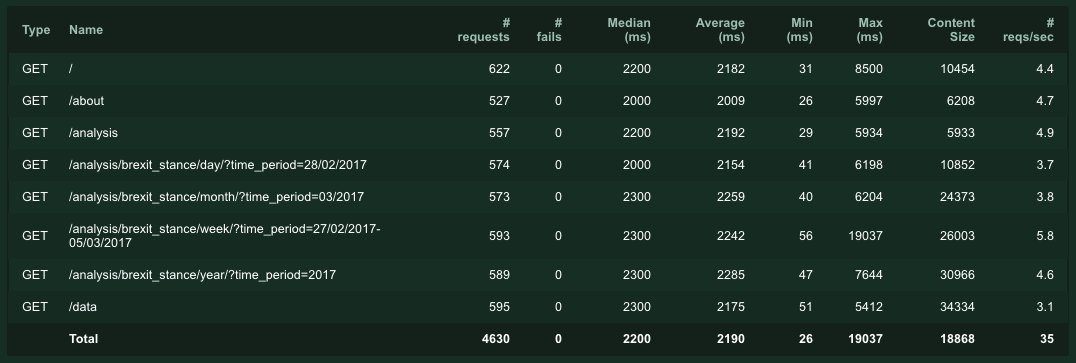
\includegraphics[width=\textwidth]{images/load-test.png}
  \captionof{figure}{Locust view of Load Testing.}
  \label{fig:locust}
\end{center}

\subsection*{Acceptance Testing}
To test against the functional and non-functional requirements identified within the Software Requirements Specification, a mix of black box and white box testing was used to comprehensively test against the set of all requirements. The result of such testing found that all requirements as identified within the system had been met. 
\\

-- See Table \ref{table:requirements} for how the System met the requirements.

-- See Table \ref{table:nonfunc-requirements} for how the System met the non-functional requirements.

\newgeometry{a4paper,left=0.75in,right=1in,top=1in,bottom=1in,nohead}
\begin{landscape}
\begin{table}[]
\centering
\label{my-label}
\begin{tabular}{ |>{\raggedright\arraybackslash}p{3.75cm}|p{1cm}|>{\raggedright\arraybackslash}p{14cm}|}
\hline
\hfil Requirement Set \hfill & REQ & Implementation  \\
\hline
\multirow{3}{*}{1. Tweet Collection} 
							   & 1.1         & The System scrapers allow for the specification of hashtags for which to collect tweets for.                                                                                           \\
							   \cline{2-3}
                                  & 1.2         & The System uses tweet selection criteria in both historic scraper and realtime scraper \\
                                 \cline{2-3}
                                  & 1.3         &  The System permanently stores the tweets it collects using the \texttt{Tweet Model} as a means of saving.\\
\hline \hline
\multirow{3}{*}{2. Tweet Tokenization} 
							   & 2.1         & The System provides a tokenization interface for manual tweet tokenization.                                                                                           \\
							   \cline{2-3}
                                  & 2.2         & The System tokenization interface accepts tweet selection criteria\\
                                 \cline{2-3}
                                  & 2.3         &  The System can tokenize a plaintext tweet into a classifiable string of tokens\\
                                  \cline{2-3}
                                  & 2.4         &  The System permanently stores the tweets it tokenizes using the \texttt{TokenizedTweet Model} as a means of saving.\\
\hline \hline
\multirow{3}{*}{3. Tweet Classification} 
							   & 3.1         & The System provides a classification interface for manual tweet classification.                                                                                           \\
							   \cline{2-3}
                                  & 3.2         & The System classification interface accepts tweet selection criteria\\
                                 \cline{2-3}
                                  & 3.3         &  The System contains a \texttt{Naive Brexit Model} and \texttt{Brexit Model} which classifies tweets on whether they are in favour (leave) or against (remain) Britain Leaving the European union \\
                                  \cline{2-3}
                                  & 3.4         &  The System contains a \texttt{Sentiment Model} wgucg classifies tweets on whether they are positive or negative towards
Britain Leaving the European union.\\
                                 \cline{2-3}
                                  & 3.5         &  The System permanently stores the tweets it tokenizes using the \texttt{TokenizedTweet Model} as a means of saving.\\
                                  \cline{2-3}
                                  & 3.6         &  The System permanently stores the tweets it classifies using the \texttt{ClassifiedTweet Model} as a means of saving.\\

\hline \hline
\multirow{3}{*}{4. Visualization} 
							   & 4.1         & The website displays all tweets the system has collected on page \texttt{data.html}.                                                                                           \\
							   \cline{2-3}
                                  & 4.2         & The System provides \texttt{analysis.html} which allows the filtering of analysis by model\\
                                 \cline{2-3}
                                  & 4.3         &  The System provides a time switcher on \texttt{classifier-analysis.html} for which analysis can be filtered by day/week/month/year\\
                                  \cline{2-3}
                                  & 4.4         &  The System displays all classifications but only a subset of top classified tweets.\\
\hline \hline
\multirow{3}{*}{5. Automation} 
							   & 5.1         & The System conducts tweet collection autonomously using the \texttt{real-time} scraper implementation.                                                                                          \\
							   \cline{2-3}
                                  & 5.2         & The System conducts tweet tokenization autonomously using asynchronous celery task \texttt{receive tweet}\\
                                 \cline{2-3}
                                  & 5.3         & The System conducts tweet classification autonomously using cron job \texttt{brexit/brexit/scripts/cron.sh} \\
                                  \cline{2-3}
                                  & 5.4         &  The System conducts tweet visualisation autonomously through dynamic \texttt{template pages}\\
\hline                                                                                                   
\end{tabular}
\caption{Requirement Implementation}
\label{table:requirements}
\end{table}
\end{landscape}
\restoregeometry % Restore the global document page margins

\begin{tabular}{ |p{2cm}||p{12.25cm}|}
 \hline
 NF-REQ & Implementation\\
 \hline
 1 & The System operates in real-time and background real-time operations occur within five minutes.\\
  \hline
 2 &   The System on average responds to HTTP requests in less than 3 seconds and has been tested with load testing.\\
  \hline
 3 & The System works across common operating systems.\\
  \hline
 4 & The System works across common browsers.\\
  \hline
 5 & The System uses JSON configuration file that allow specifying models.\\
  \hline
 6 & The System uses Django's data models which are extensible through South Migrations.\\
  \hline
 7 & The System uses supervisor to ensure it is reliably up and operating.\\
 \hline
\end{tabular}
\captionof{table}{Non-Functional Requirement Implementation}
\label{table:nonfunc-requirements}

\subsection*{Continuous Integration}
For the automated checking of the formally written unit and integration tests within the system the continuous integration environment \textit{Jenkins} was used. Jenkins as previously mentioned within \textit{Section \ref{sec:deployment}} allows for the specification of a delivery pipeline, for ensuring System correctness during deployments a test step was put into the pipeline. Upon executing the test step of the delivery pipeline, each of the tests contained in the System is run against the new System to ensure the previous behaviour of the System is upheld when new changes have been implemented. If the tests fail within the execution of the test step, Jenkins records the build as a fail, and the deployment is abandoned allowing for the problematic changes to be caught early. Continuous integration ensures the system can be tested in a clean environment (created by the build step) on the Jenkins server thus providing confidence in the functionality of the System as the Jenkins environment is reflective of that of the final destination of the remote local production server. See Figure \ref{fig:test-trend} for the Jenkins view of continuous integration testing of previous deployments through a test result trend chart.

\begin{center}
  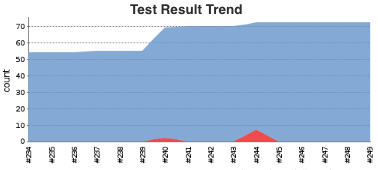
\includegraphics[width=0.6\textwidth]{images/test-trend.png}
  \captionof{figure}{Jenkins view of Continuous Integration testing of deployments.}
  \label{fig:test-trend}
\end{center}
\end{document}

\documentclass[11pt]{report}
\usepackage{standalone}
\graphicspath{ {images/} }
\setcounter{tocdepth}{5}
\setcounter{secnumdepth}{5}
\usepackage{natbib}
\usepackage{bibentry}
\bibliographystyle{agsm}
\usepackage{etoolbox}
\setlength{\parindent}{0em}
\setlength{\parskip}{0.25em}
\usepackage[raggedright]{titlesec}
\usepackage{hyperref}
\usepackage{capt-of}
\patchcmd{\bibliography}{\section*}{\section}{}{}
\titlespacing*{\chapter}{0pt}{-40pt}{10pt}
\titleformat{\chapter}[block]{\normalfont\huge\bfseries}{\thechapter}{15pt}{}
\usepackage{rotating}
\usepackage[titletoc]{appendix}
\usepackage{pgfgantt}
\usepackage{graphicx, rotating, caption, lscape, threeparttable}% \usepackage{amsmath}
\usepackage{array}
\usepackage{pdflscape}
\usepackage{geometry}
\usepackage{listings}
\usepackage[T1]{fontenc}
\usepackage[bottom]{footmisc}
\usepackage{subcaption}
\usepackage{float}




\begin{document}
\chapter{Discussion}

\section{Findings}

\subsection*{Quality of Data}
As the System collects its own data for classification it is worth reviewing the quality of this input data. Initially the System was going to be designed with a fully fledged Twitter API but due to the constraints of limited backdating of Twitters' tweets the historic HTML scraper of GetOldTweet's python was integrated. HTML scraping is subject to problems of rate-limiting, malformed scraping and document object model changes. Unfortunately, during the development of the System all of these problems occurred. Rate-limiting of the HTML scraping occurred early within data collection delaying progress for forming the dataset. Some of the returned tweets were also found to be malformed, specifically tweets with URL's as the URL was being incorrectly parsed from the HTML document object model (DOM). Finally, the historic scraper during the backdating of tweets became subject to a change in twitter's HTML DOM structure of the page causing unexpected behaviour within the running of the scraper. As a counter measure, a fix was implemented for this and was even integrated into the git repository of the scraper for the open source community to benefit from the fix also \footnote{Open Source contribution accessible via https://github.com/Jefferson-Henrique/GetOldTweets-python/commit/b9d5a1d21256832ceba797ab8b8b421e8572618a}.
\\

Towards the end of the development of the System the real-time scraper Tweepy was also integrated into the System. The System now had two sources of tweet data and the differences between the api's became apparent. Tweepy provided consistently more tweets, with a large amount of those tweets being retweets (\textit{tweets that are reposted and prefixed with RT}). These extra retweets all seemed to be truncated with `...' where the length of the retweet is too long. These points although small can effect the overall classification of a tweet, and thus is worth noting when comparing analysis computed by the system prior to the integration of Tweepy.
\\

Despite notions of inefficiency in data collection, both the historic and real-time scrapers were successfully integrated into the final System. The result of such integrations has allowed the System to collect a vast amount of data (see Table \ref{table:tweet-stats} for overall statistics) with the produced dataset having prospect of being made publicly available for others to use (after the publishing of this report).
\\
\vspace{-0.5cm}
\enlargethispage{\baselineskip}

\begin{center}
\begin{tabular}{ |p{2cm}||p{2cm}|}
 \hline
 Tweets & Users\\
 \hline
 7,110,544 & 1,210,824 \\
 \hline
\end{tabular}
\captionof{table}{Tweet Collection Statistics \textbf{as of publishing date}}
\label{table:tweet-stats}
\end{center}
\clearpage

\subsection*{Quality of Classifications}

Despite the large amount of data being collected from the brexit hashtags, the amount of training data available to the classifiers was a small proportion. The decision was also taken to improve the classification accuracy by exempting tweets containing malformed URL's (i.e. URL's that could not be replaced via a regular-expression) and tweets containing images from the classification process as it could be argued to be harder to extract sentiment from these tweets. Therefore, the small proportion training set became even smaller from the exemption of tweets. The Naive Brexit Model still achieved a noteworthy average accuracy of 70\% however the Sentiment Model wasn't as accurate; only achieving 66\% somewhat responsible to it's weaker and smaller training set of 6096 tweets compared to the 22,120 tweets of the Naive Brexit Model. Bootstrapping an existing labelled tweet dataset for training the sentiment model was also an option however the preference of domain training data over generalized was chosen instead. 
\\

The classifications computed by the Naive Brexit model performed well on clear cut distinctions that encouraged or discouraged ``Britain leaving the European Union'' which can be seen in the correctly classified Brexit tweet section of Appendix A. Tweets which discussed being `out' or talked in the tense of having `left' were correctly classified as discussing leave. Where Tweets that discussed remaining or discussed leave associated phrases with a negative tone were classified as remain. However tweets which were sarcastic led to inaccurate classifications like the tweet in incorrectly classified Brexit tweets section of Appendix A. Neutral tweets also existed such as news stories and count down timers for Brexit commencement so these were misclassified as they didn't really belong to either of the classes which makes the case for whether the model should have been trained as a multinomial classifier containing a neutral classification rather than a binomial. Tweet's of a limited length also proved a problem to classification, ``Die hard \#Brexit'' only provides two words for classification after tokenization (removal of the hashtag) and thus the confidence in classification of this tweet was just over random distribution at 50.001\%
\\

The Sentiment model classifications performed well on tweets that were assertive or pessimistic towards ``Britain leaving the European Union'' which can be seen in the correctly classified Sentiment tweet section of Appendix A. Tweets that mentioned `regret' or condemned past and future events regarding brexit were correctly classified as being negative. Where Tweets that were humorous or contained assertive support tended to be classified correctly as positive. Again the same neutrality occurs this time in the overall emotion of the tweet is (see Incorrectly Classified Sentiment Tweets in Appendix A). Tweets which gave connotations of both classes were also incorrectly classified e.g. the same tweet contained the phrase ``A Huge Thank you to everyone for their superb and supportive'' and ``we must fight'' but was classified as negative despite the overall tone being narrowly more positive.
\\

Tweets outside of the topic of discussion were also collected, the likes of the recent American Presidential Elections adopted the hashtag ``\#StrongerTogether'' and various tweets had the Systems Brexit defined hashtags with content that was not at all related to the hashtags (see Offf Discussion Topic Tweets in Appendix A). The result of classifying these irrelevant tweets is the skew of overall classification statistics and is worth noting. It was due to the observation of changing use of hashtags that a very specific and limited subset of hashtags were actually used in formulating the training set of the Naive Brexit Model.

\subsection*{Test Coverage}
Due to time constraints within the project and complexity of various technologies, there is testing missing from some classes that entail spinning off new threads and thus prove harder to test. These classes such as the \texttt{BatchClassificationService} class have however been tested manually and walked through via an Django debugger to verify behaviour.


\subsection*{Results}
The results of the analysis found that volume of leave tweets (blue) was consistently higher than the volume of remain tweets (red) and the volume of positive tweets (green) was also consistently higher than negative ones (red). (see Figures \ref{fig:naive-results}, \ref{fig:brexit-results} and \ref{fig:sentiment-results} ). 
\\

\textit{N.B. all of the model result figures below were extracted from the System's website}

\begin{figure}[H]
        \begin{subfigure}[b]{0.33\textwidth}
                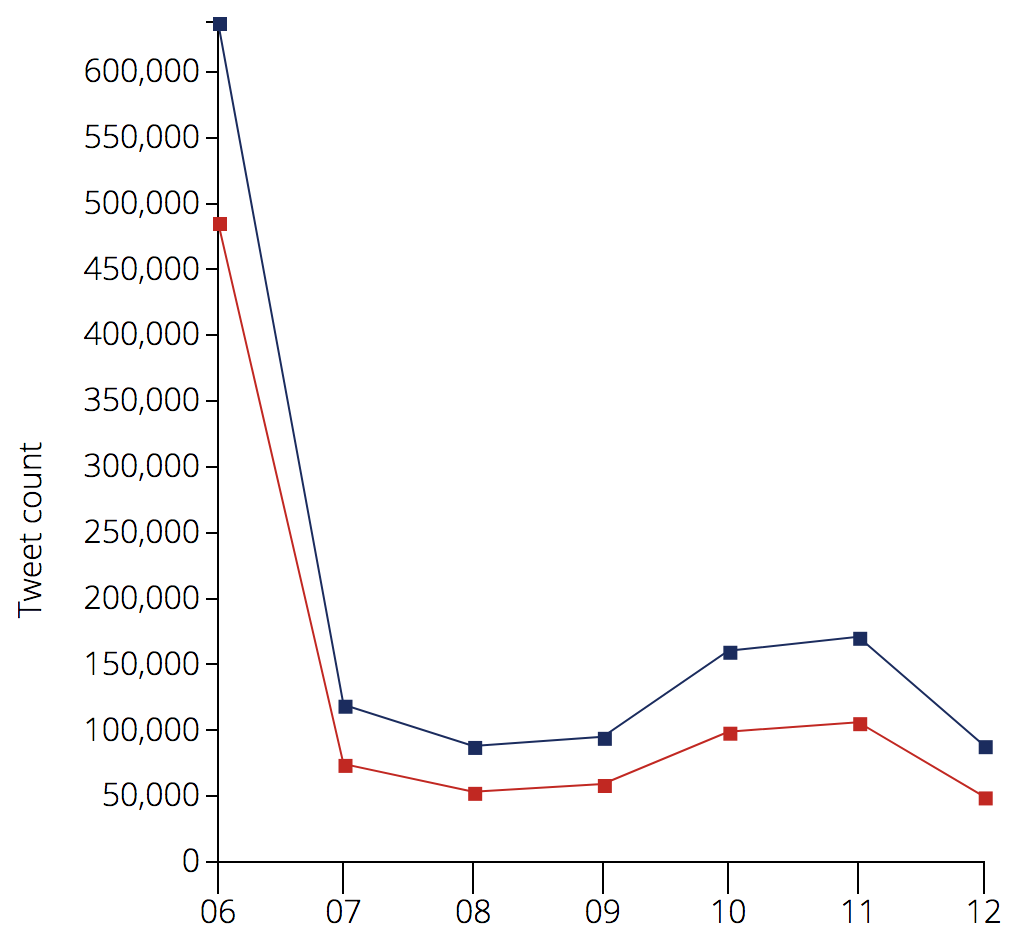
\includegraphics[width=\linewidth]{images/2016-naive.png}
                \caption{2016}
                \label{fig:gull}
        \end{subfigure}%
        \begin{subfigure}[b]{0.33\textwidth}
                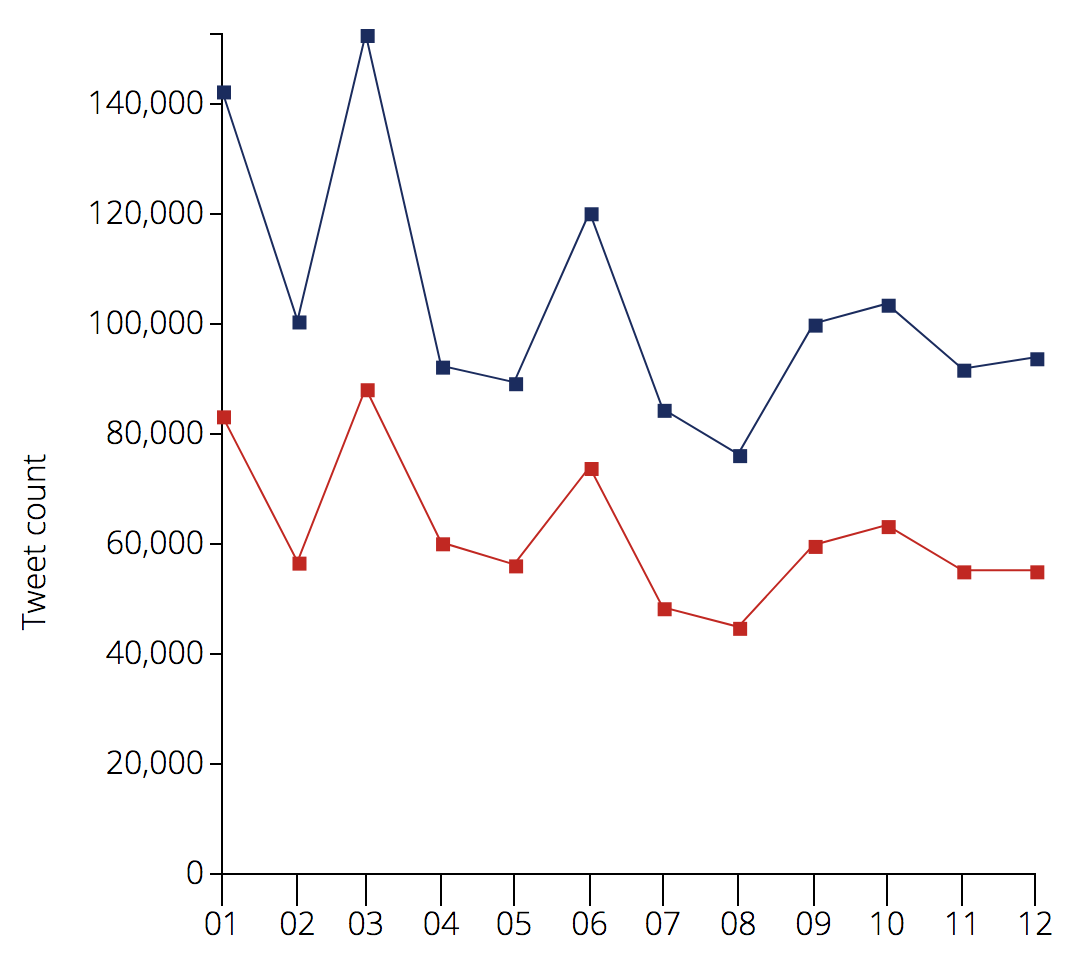
\includegraphics[width=\linewidth]{images/2017-naive.png}
                \caption{2017}
                \label{fig:gull2}
        \end{subfigure}%
        \begin{subfigure}[b]{0.30\textwidth}
                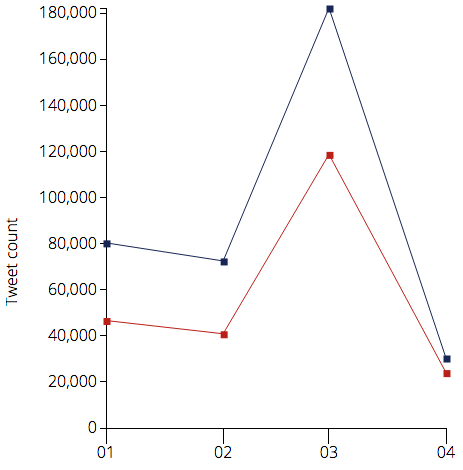
\includegraphics[width=\linewidth]{images/2018-naive.png}
                \caption{2018}
                \label{fig:tiger}
        \end{subfigure}%

        \caption{Naive Brexit Stance Model Results}\label{fig:naive-results}
\end{figure}

\begin{figure}[H]
        \begin{subfigure}[b]{0.35\textwidth}
                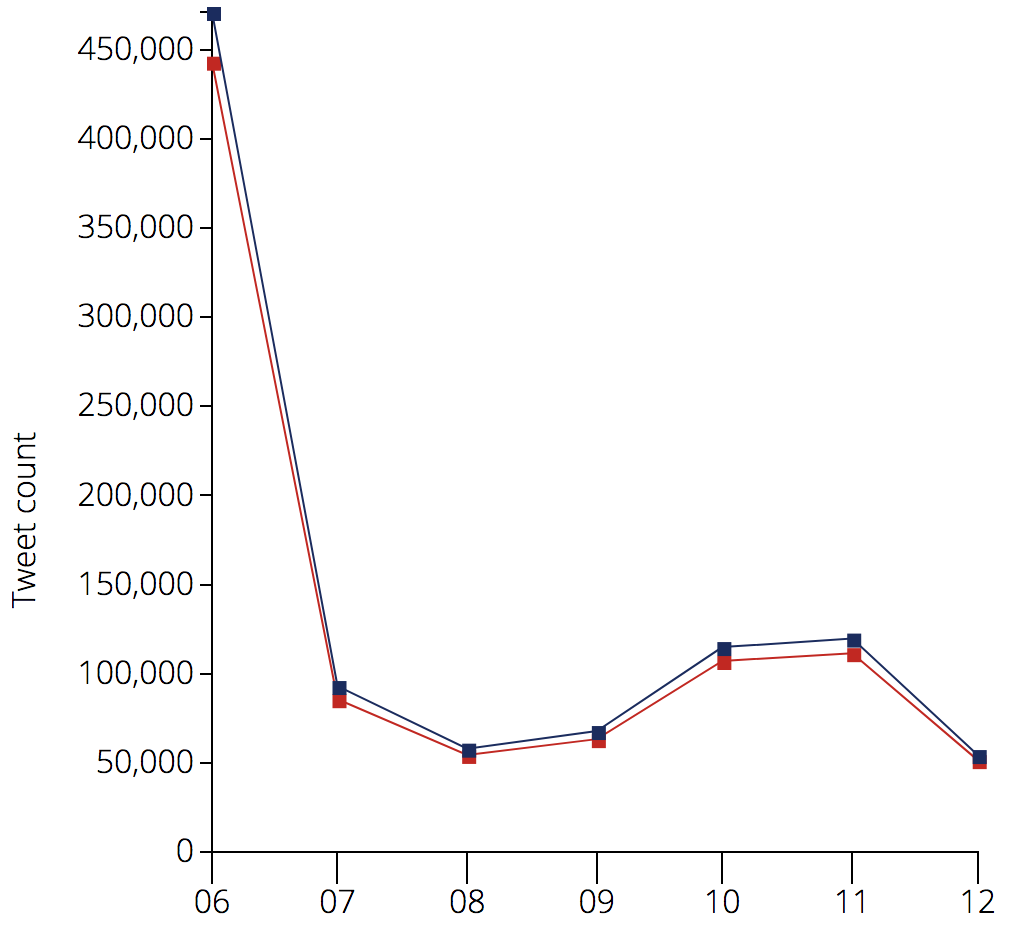
\includegraphics[width=\linewidth]{images/2016-brexit.png}
                \caption{2016}
                \label{fig:gull}
        \end{subfigure}%
        \begin{subfigure}[b]{0.33\textwidth}
                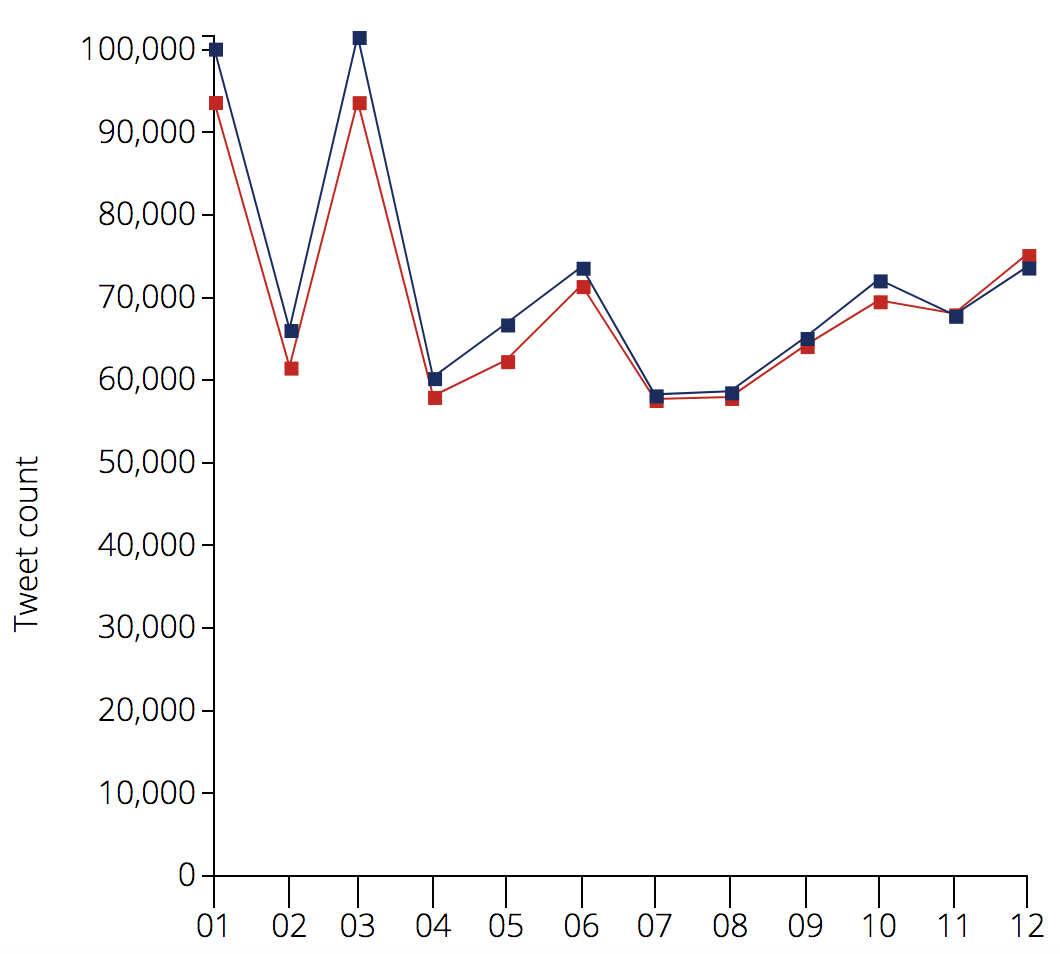
\includegraphics[width=\linewidth]{images/2017-brexit.png}
                \caption{2017}
                \label{fig:gull2}
        \end{subfigure}%
        \begin{subfigure}[b]{0.30\textwidth}
                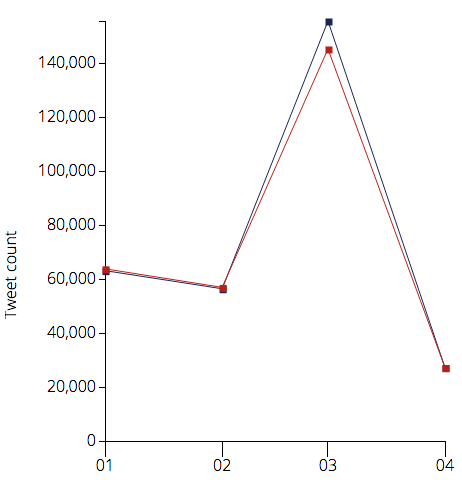
\includegraphics[width=\linewidth]{images/2018-brexit.png}
                \caption{2018}
                \label{fig:tiger}
        \end{subfigure}%

        \caption{Brexit Stance Model Results}\label{fig:brexit-results}
\end{figure}

\begin{figure}[H]
        \begin{subfigure}[b]{0.35\textwidth}
                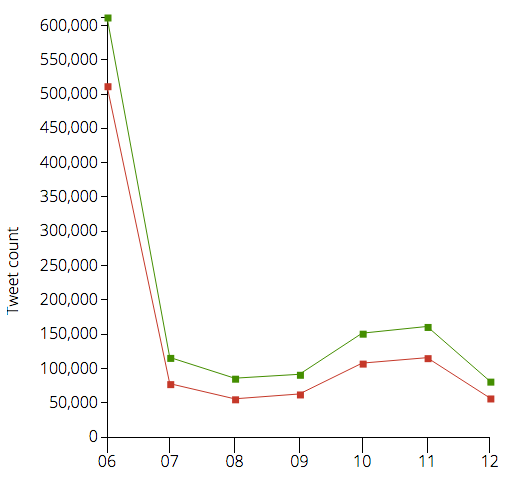
\includegraphics[width=\linewidth]{images/2016-sentiment.png}
                \caption{2016}
                \label{fig:gull}
        \end{subfigure}%
        \begin{subfigure}[b]{0.33\textwidth}
                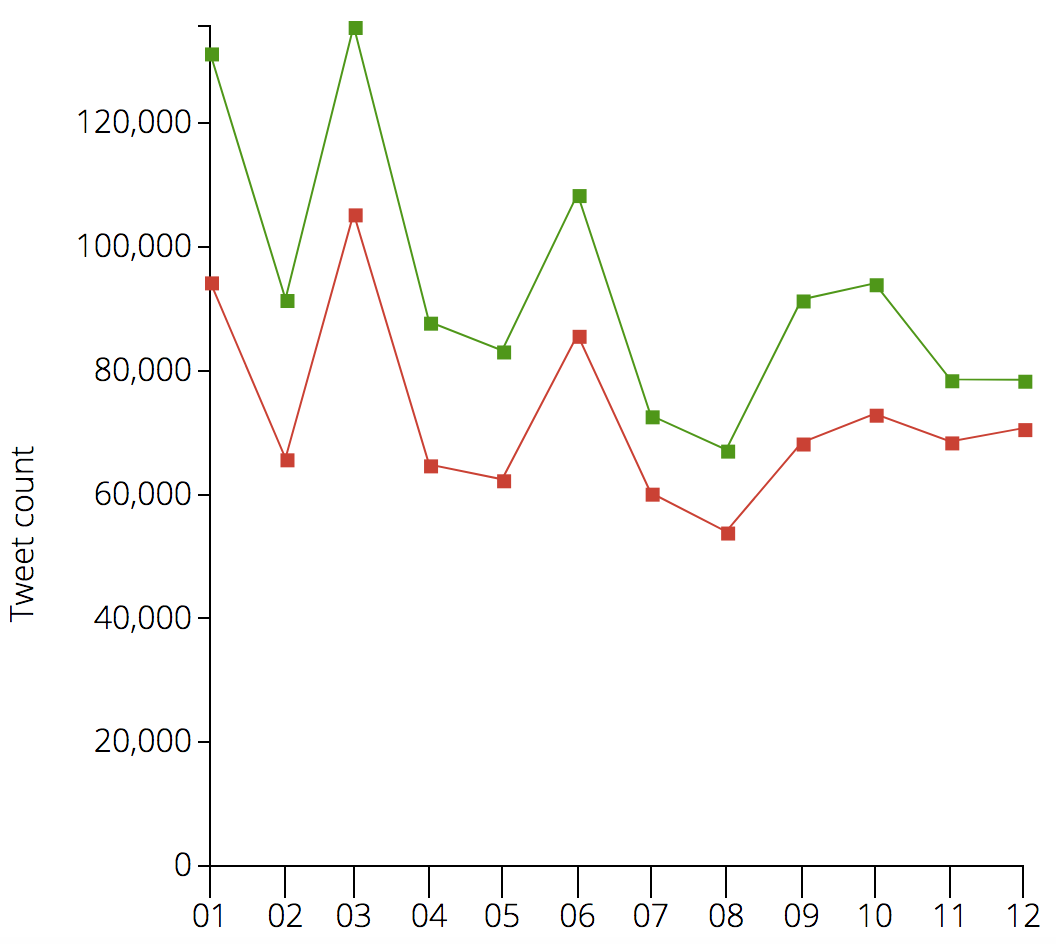
\includegraphics[width=\linewidth]{images/2017-sentiment.png}
                \caption{2017}
                \label{fig:gull2}
        \end{subfigure}%
        \begin{subfigure}[b]{0.30\textwidth}
                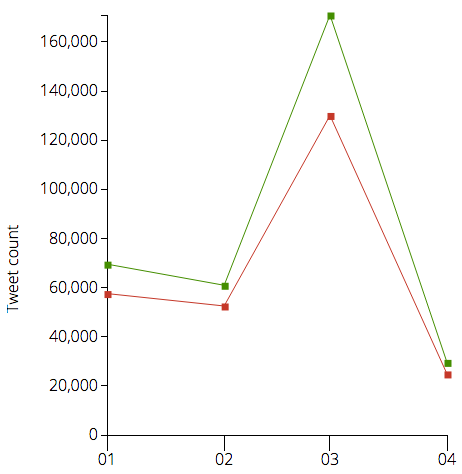
\includegraphics[width=\linewidth]{images/2018-sentiment.png}
                \caption{2018}
                \label{fig:tiger}
        \end{subfigure}%

        \caption{Sentiment Model Results}\label{fig:sentiment-results}
\end{figure}

\subsection*{Performance}
The System's two time consuming operations are the tokenization and classification of tweets. Through testing of the System on a computer with a 2.7 GHz Intel Core i5 dual core processor and three threads available to the System; it achieved 320 tokenizations per second and 280 classifications per second. On computers of a higher specification, the thread number could be higher and thus would result in a higher rate per second for both operations.


\subsection*{System Comparison}
The final System can be compared to the Brexit Systems mentioned within the related work. Table \ref{table:comparison} shows how the System developed within this report compares to the Edinburgh \citep{llewellyn_brexit?_2016} and Sheffield \citep{maynard_framework_2017} Systems. The results show that the System developed as part of this paper has incrementally improved on the current Systems that have analysed Brexit.

\begin{center}
\begin{tabular}{ |p{3cm}||p{2cm}|p{2cm}|p{2cm}|}
 \hline
 System & Real-Time & Machine Learning & Deep-Learning\\
 \hline
  Edinburgh & Yes & No & No \\
 \hline
 Sheffield & Yes & Yes & No \\
  \hline
 Our System & Yes & Yes & Yes \\
 \hline
\end{tabular}
\captionof{table}{System Comparison.}
\label{table:comparison}
\end{center}



\section{Future Work}
During the inception of the project there was scope to implement a variety of aspects to the real time sentiment analysis system. However, due to the time constraints of the project it was necessary to hone in on the detailed implementation of the System Features as identified within this report. This therefore leaves the below list of features that would provide ideal extensions to the system.

\begin{itemize}
\item Baseline Comparison: The System confidence in classification accuracy would benefit off of the implementation of a baseline accuracy through an SVM classifier rather than the existing comparison of a random distribution accuracy.

\item Online Learning: The Systems models were trained on small sample sizes due to the amount of data available at the time of training. As the System continuously collects tweets an extension would be to have the System retrain it's classification models when new training data becomes available thus learning in an online fashion.
 
\item Emotion Classification: As the System can easily integrate new classification models, predicting the Emotion of tweets could be added as a model. The model would classify tweets regarding Brexit using a six point mood scale \citep{pepe_between_2008} and would allow for the extraction of more analysis into sentiment on the issue. Thus as an extension the System could have a model which is classified on the distant labelling of emotions categories.
\end{itemize}

\end{document}

\documentclass[11pt]{report}
\usepackage{standalone}
\graphicspath{ {images/} }
\setcounter{tocdepth}{5}
\setcounter{secnumdepth}{5}
\usepackage{natbib}
\usepackage{bibentry}
\bibliographystyle{agsm}
\usepackage{etoolbox}
\setlength{\parindent}{0em}
\setlength{\parskip}{0.25em}
\usepackage[raggedright]{titlesec}
\usepackage{hyperref}
\usepackage{capt-of}
\patchcmd{\bibliography}{\section*}{\section}{}{}
\titlespacing*{\chapter}{0pt}{-40pt}{10pt}
\titleformat{\chapter}[block]{\normalfont\huge\bfseries}{\thechapter}{15pt}{}
\usepackage{rotating}
\usepackage[titletoc]{appendix}
\usepackage{pgfgantt}
\usepackage{graphicx, rotating, caption, lscape, threeparttable}% \usepackage{amsmath}
\usepackage{array}
\usepackage{pdflscape}
\usepackage{geometry}
\usepackage{listings}
\usepackage[T1]{fontenc}
\usepackage[bottom]{footmisc}
\usepackage{multirow}
\usepackage{float}
\usepackage{subcaption}



\usepackage{etoolbox}
\usepackage{epigraph}

\setlength\epigraphwidth{11cm}
\setlength\epigraphrule{0pt}
\makeatletter
\patchcmd{\epigraph}{\@epitext{#1}}{\itshape\@epitext{#1}}{}{}
\makeatother


\begin{document}
\chapter{Conclusion}

The textual content of social media posts, in particular tweets; contain a rich source of polarised opinion that can be utilized in the Sentiment Analysis of a domain area. This dissertation has combined the method of Sentiment Analysis with tweets posted in real-time on Twitter to validate that we can indeed `implement an autonomous system to extract and visualise public sentiment from Tweets within sufficient real time'. Using the case study of the Twitter debate on ``Britain leaving the European Union'' the System has collected, analysed and visualized the sentiment of individuals within real-time. Improving on previous Systems, the utilization of Machine Learning techniques through the implementation of deep-learning models in this System has shown that deep-learning can be used in the determination of a users' sentiment within a tweet and the classification of tweets using this method can be accomplished within real-time. The enclosed work within this dissertation highlights the design, implementation and issues around the development of a real-time Sentiment extraction System and can thus be used as a reference point for future Systems of this class.
\end{document}
\clearpage




\addcontentsline{toc}{chapter}{Bibliography}
\bibliography{references/refbiblatex}

\clearpage

\addappheadtotoc
\appendix

\addcontentsline{toc}{section}{Appendix A. System Classified Tweets}
\documentclass[11pt]{report}
\usepackage{standalone}
\graphicspath{ {images/} }
\setcounter{tocdepth}{5}
\setcounter{secnumdepth}{5}
\usepackage{natbib}
\usepackage{bibentry}
\bibliographystyle{agsm}
\usepackage{etoolbox}
\setlength{\parindent}{0em}
\setlength{\parskip}{0.25em}
\usepackage[raggedright]{titlesec}
\usepackage{hyperref}
\usepackage{capt-of}
\patchcmd{\bibliography}{\section*}{\section}{}{}
\titlespacing*{\chapter}{0pt}{-40pt}{10pt}
\titleformat{\chapter}[block]{\normalfont\huge\bfseries}{\thechapter}{15pt}{}
\usepackage{rotating}
\usepackage[titletoc]{appendix}
\usepackage{pgfgantt}
\usepackage{graphicx, rotating, caption, lscape, threeparttable}% \usepackage{amsmath}
\usepackage{array}
\usepackage{pdflscape}
\usepackage{geometry}
\usepackage{listings}
\usepackage[T1]{fontenc}
\usepackage[bottom]{footmisc}


\begin{document}
\section*{Appendix A. System Classified Tweets}

\subsection*{Correctly Classified Brexit Tweets}

\subsubsection*{Tweets Classified Leave}
-- ``Out of sheer envy the EU mandated that we pay \pounds1.7bn worth of contributions in 2014 wishing to free-load on our economic success. After all we procure goods from them. Now they set a figure within the region of \pounds40bn. What justifies this farcical calculation \#Brexit''

-- ``Get over it, we're on our way out \#Brexit''

\subsubsection*{Tweets Classified Remain}
-- ``How much of a hit to the economy would you take to prevent foreigners coming to the UK? \#Remain''

--``The economic and political cost of UK austerity \#Brexit \#FBPE \#StopBrexitSaveBritain \#FinalSay http://bit.ly/2FQhHwo''
\subsection*{Incorrectly Classified Brexit Tweets}

\subsubsection*{Tweets Classified Leave}
--``Yeah, \#Brexit .....because it's so much easier to negotiate trade deals with big powerful countries when you're not part of a powerhouse trading block! Oh, wait....''

\subsubsection*{Tweets Classified Remain}
--``Brexit is 9527 hours away. \#brexit''

-- ``Die hard \#Brexit''

\subsection*{Correctly Classified Sentiment Tweets}

\subsubsection*{Tweets Classified Positive}
-- ``This is an interesting point. First of all, we need another election, and soon. Then maybe we can get to where \#Brexit can be re-considered.''

-- ``Looking forward to see what last-minute deal the UK will offer the Republic not to veto its \#Brexit negotiations with the EU. Any offer they make will be of great interest, especially in the instance Scotland revisits the question of whether it wants to be independent again.''

\subsubsection*{Tweets Classified Negative}
-- ``Angela Merkel's open-door policy CAUSED the migrant crisis led to \#brexit in \#eu , furious George Soros blasts http://shr.gs/suCTcuW''

-- ``It has been said that you should, "Never trust a Tory." So why should it be any different during the Brexit negotiations? \#BrexitMeansBrexit \#BrexitPerversion \#Brexit \#MayMustGo https://youtu.be/CZ4lhmARnCc''

\subsection*{Incorrectly Classified Sentiment Tweets}

\subsubsection*{Tweets Classified Positive}
-- ``Stop being so negative. Get behind \#brexit and be positive. You're ignoring the will of the people. They elected May and Tories. You're an A Grade Bremoaner''

-- ``No. That's precisely the point. That's the deception here. It's totally and utterly clear that \#Corbyn is a \#Brexiter and that he and @UK Labour WILL deliver \#Brexit come what may. He has said so - repeatedly. There will be no u-turn. That's why it's \#Remain OR \#Labour''

\subsubsection*{Tweets Classified Negative}
-- ``RT @conorwells0: A Huge Thank you to everyone for their superb and supportive comments since I switched from Leave to Remain, we must fight...''

--``@David\textunderscore Cameron Put this poster in your window and send local politicians a message. \#Brexit https://t.co/6cxCsZKhSv''


\subsection*{Off Discussion Topic Tweets}
-- ``How the NRA uses an app to organize opposition to gun control via @Salon \#Brexit \#StopBrexit https://buff.ly/2CjFXs8''

-- ``Greece needs capital, ingenious Irish biscuits and mince pies. \#ExportOpps \#TakeBackControl''

--`\#ButHerEmails -> WAR \#RussiaGate \#Assange \#Putin \#InfoWars \#Trump \#Breitbart \#AlexJones \#Murdoch \#Mercer \#Brexit \#Milo \#Forage Alt-right https:// twitter.com/angryblacklady /status/895279622983516160 …''

\end{document}


\addcontentsline{toc}{section}{Appendix B. File Structure}
\addcontentsline{toc}{section}{Appendix C. System Usage}
\clearpage

\documentclass[11pt]{report}
\usepackage{standalone}
\graphicspath{ {images/} }
\setcounter{tocdepth}{5}
\setcounter{secnumdepth}{5}
\usepackage{natbib}
\usepackage{bibentry}
\bibliographystyle{agsm}
\usepackage{etoolbox}
\setlength{\parindent}{0em}
\setlength{\parskip}{0.25em}
\usepackage[raggedright]{titlesec}
\usepackage{hyperref}
\usepackage{capt-of}
\patchcmd{\bibliography}{\section*}{\section}{}{}
\titlespacing*{\chapter}{0pt}{-40pt}{10pt}
\titleformat{\chapter}[block]{\normalfont\huge\bfseries}{\thechapter}{15pt}{}
\usepackage{rotating}
\usepackage[titletoc]{appendix}
\usepackage{pgfgantt}
\usepackage{graphicx, rotating, caption, lscape, threeparttable}% \usepackage{amsmath}
\usepackage{array}
\usepackage{pdflscape}
\usepackage{geometry}
\usepackage{listings}
\usepackage[T1]{fontenc}
\usepackage[bottom]{footmisc}


\begin{document}
\section*{Appendix B. File Structure}
The zip file submitted as fulfilment of this project contains the git-repository, and the report PDF that you are currently reading.Within the \texttt{git-repository/} folder there is the system contained in the \texttt{brexit/} folder and the files which make up the report in the \texttt{report/} folder.
\section*{Appendix C. System Usage}
The System uses an AWS database which is currently under paid subscription so as a measure of restricting usage of this, the access to the System has been restricted and thus \textbf{viewing the System must occur via UoBWifi or eduroam wifi connection}.
\\

System URL: http://www.senticle50.co.uk/

Jenkins URL: http://www.senticle50.co.uk:8080/
\\

For running the system locally see ReadMe.md contained within the \texttt{git-repository/} folder.
\end{document}


\end{document}